\documentclass[review]{elsarticle}

\usepackage{lineno,hyperref}
\usepackage{amsmath,amsfonts}

\usepackage[plain]{algorithm}
\usepackage[noend]{algpseudocode}
\renewcommand{\algorithmiccomment}[1]{{\quad\footnotesize // #1}}
\renewcommand{\algorithmicrequire}{\textbf{Input:}}
\renewcommand{\algorithmicensure}{\textbf{Output:}}

\modulolinenumbers[5]

\journal{Biologically Inspired Cognitive Architectures}

%\bibliographystyle{elsarticle-num}
\bibliographystyle{model5-names}\biboptions{authoryear}
%%%%%%%%%%%%%%%%%%%%%%%

\begin{document}

\begin{frontmatter}

\title{Behavior Planning of Intelligent Agent with Sign World Model}

%% Group authors per affiliation:
\author{Aleksandr I. Panov\corref{corauth}}
\ead{pan@isa.ru}

\cortext[corauth]{Corresponding author}
\address{Federal Research Center ``Computer Science and Control'' of RAS, Moscow, Russia\\
National Research University Higher School of Economics, Moscow, Russia}

\begin{abstract}
Behavior planning is an important function of any complex technical facility intelligent control system. Presently, a symbol paradigm of artificial intelligence offers a variety of planning algorithms, including those that use precedent information, i.e. algorithms based on acquired knowledge. A symbol grounding problem within the exiting approaches of knowledge representation does not allow effective use the developed algorithms together with learning mechanisms for the purpose of solving a wide variety of applied problems by actual intelligent agents (robotics systems). This article presents the original planning algorithm (MAP Planner), which uses a sign world model as the basis for acquisition and maintenance of knowledge for future use in behavior planning. the sign problem approach describes planning as a cognitive function actualized by the world model of a subject of activity. Apart from solving symbol grounding problems and ensuring psychological and biological plausibility, a sign planning process model allows interaction of an intelligent agent with other participants in solving a cooperative task. The article presents the description of the knowledge representation method used, a MAP planning algorithm, and a model experiment in a ``block world''.
\end{abstract}

\begin{keyword}
behavior planning \sep sign world model \sep sign image \sep sign significance \sep sign personal meaning \sep causal matrix \sep semiotic network \sep MAP algorithm \sep case-based planning
\end{keyword}

\end{frontmatter}

\linenumbers

\section{Introduction}\label{sec:intro}

The issue of behavior planning of a complex technical or virtual subject has a long history and is mainly associated with the successes in specific area of the Artificial Intelligence discipline --- automatic planning. In this sphere, considerable success has been achieved and a number of sign-based planning methods were proposed --- both for classical problem definition, where actions are deterministic (these are such planning algorithms as FF \cite{Hoffmann2001}, FD \cite{Helmert2006}, LAMA \cite{Richter2010}), and in non-deterministic definition, which takes into consideration the nonzero probabilities of non-appliance of actions and probabilistic environment reaction (algorithms based on Markov processes and dynamic programming \cite{Barto1995,Bonet2009}). However, the development of effective and fast planning algorithms is based on the preset heuristic graph search principles and on the assumption that a set of actions is known in advance, which makes a planning system’s automatic adaptation to new problems with a new list of actions impossible. This implies that classical approaches do not offer a carry-over of planning experience or abstract actions, which may have varying realizations in different situations. Substantial challenges arise when the existing algorithms are adapted for multi-agent applications, which suggests that agents possess both different action sets and different knowledge of the environment \cite{Brafman2015}. In case of cooperative interaction, it is also necessary to ensure non-discretionary incorporation of learning elements to augment the database of an agent with information supplied by other participants of the group.

In more recent times, researchers in the fields of control and planning theory have focused on psychologically and biologically inspired models and architectures of agent control \cite{Kelley2006,Sun2012a}. The use of different types of memory (episodic, procedural, etc.) in cognitive architectures is aimed exactly at solving the task of reproducing biological and psychological methods of information interchange and organization to solve such problems as behavior control and planning. This is primarily driven by the fact that the increasing complexity of tasks performed by robotics systems (agents) requires their higher self-sufficiency, versatility, and flexibility, which the existing methods and algorithms are unable to provide. Researchers in the field of Artificial Intelligence once again turn to the natural examples of such problem solving --- to the research of human and animal behavior \cite{Redko2016,Panov2016b}. Psychologically inspired models of cognitive functions (including planning) are focused both on reproducing human behavior in complex, specifically cooperative conditions, and at complying, as fully as possible, with the existing psychological concepts of human mind functioning. On the one hand, this may result in an increased resource intensity of the proposed algorithms, but, on the other hand, it will allow a realization of new possibilities, which previously had been left out of the scope of problems tackled by planning specialists, such as goal-setting or role designation capacity. In the past, cognitive psychology concepts have been also used in classical planning; however, mainly in behavioristic agendas. For instance, the concept of dividing the entire multiplicity of actions into automatic, fast actions, specific, voluntary actions and generalized actions predicted by psychological theory \cite{Kahneman2011} was implemented by hierarchical planning and the concept of planning experience maintenance --- in precedent planning \cite{Hammond1990,DeLaRosa2013,Borrajo2015}.

Cognitive psychology has a number of branches that study the phenomenon of planning, within which three main areas should be mentioned: planning as part of a cognitive scheme \cite{Neisser1976}, planning as a meta-process \cite{Flavell1979,Sternberg2000} and planning as part of an activity \cite{Leontyev2009}. The first branch uses cognitive schemes to describe behavior of humans. For example, a perceptive scheme is a program of gathering information about objects and events, as well as acquisition of new information to provide its consistent interpretation. The scheme simultaneously incorporates a plan and its implementation; it is both an actionable structure and a structure of actions. The second approach provides for the existence of metacognitive processes allowing a person to control his/her cognitive processes and knowledge. From Sternberg's point of view, one may talk about global (strategic) and local (tactical) planning. Global planning requires more time, but this is compensated by the reduction of time dedicated to local, tactical planning. Finally, the third approach, which is one of the most general concepts, considers hierarchical activity theory. This theory is used in this article and is described in the following section. 

It is also worth mentioning that psychologically and biologically inspired control and planning models provide a new perspective to the symbol grounding problem \cite{Harnad1990,Barsalou1999,Chella2003,Besold2015}. Neurophysiological models of brain cortex sensor region functioning together with psychological categorization and perception theory form the basis for the development of new consistent models of association of symbols and sensor data. Success in this field has made it possible to implement certain models in robotic systems \cite{Heintz2010}. 

This article will present a new psychologically and biologically inspired method of behavior planning based on sign theory of activity and structural models of cortical-thalamic regions of brain. Apart from its value in terms of modeling of human cognitive functions, sign approach may be used to solve a number of cooperative robotics problems (e.g., for intelligent movement problems \cite{Panov2016b,Panov2016c}), which cannot be solved by classical or other psychology-oriented methods (such as BDI \cite{Sardina2006}).

The main purpose of the article is to demonstrate the sign approach for modeling of such an important cognitive process as a behavior planning. The proposed planning method (MAP-algorithm) does not build more efficient plans than other existing planners and is faced with the same problems (such as a Sussman anomaly). Also considered is that MAP-algorithm does not use all components of a sign leading to a simplified model similar to a frame approach and rule systems. However, inclusion of the learning process and another components of the sign enables us to describe the goal setting process and models of coalition formation \cite{Skrynnik2016,Osipov2014c}.

This article is further organized as follows: Section \ref{sec:swm} introduces the main concepts used in the article: a world model, as well as a sign and its components are defined and substantiated from psychological and biological standpoint. Subsection \ref{subsec:components} introduces the concept of a causal matrix as a mathematical structure for the description of sign components and considers its main characteristics. Subsection \ref{subsec:causal_net} discusses the networks, which are formed on the basis of sets of causal matrices and which represent relations of sign components. Section \ref{sec:semiotics} introduces the concept of semiotic network as a model of world model and discusses the main types of processes of activity propagation within a semiotic network. Section \ref{sec:plan} presents the description of a MAP algorithm of behavior planning in a sign world model (in a semiotic network). Section \ref{sec:example} concludes with a model example of operation of the presented MAP Planner.


\section{Sign World Model}\label{sec:swm}

In this article, the method of knowledge representation is based on a sign world model  \cite{Osipov2014c,Osipov2015d, Osipov2015c}, which both stores knowledge about objects, processes and relations of external environment and represents the internal parameters of the intelligent agent that determine its motivational constituent and activity experience. The world model also includes the procedures of operation with knowledge, its acquisition and its use in various processes, such as perception, reasoning, goal-setting and behavior planning \cite{Osipov2015d}. The representation of the world model is based on psychological concepts of human brain functioning, in particular on the concepts of cultural and historical approach \cite{Vygotsky1986}, activity theory \cite{Leontyev2009,Verenikina,Igira2009} and dual systems \cite{Evans2013,Stanovich2009}. According to psychological views, a world model component is a four-element structure: a sign, which represents all entities of external environment and inner space for the subject (in our case, an intelligent agent); objects and their properties; processes; and relations between objects and processes. It should be noted that a sign is a product of interaction between several subjects of activity forming a certain group (a cultural environment), thus, the concept of a sign inherently assumes that an individual's world model interacts with the world models of other individuals.

Below we will give informal definitions and examples of a sign and each ща its components and then introduce a formal structure (causal matrix) (see subsection \ref{subsec:components}) to define all of them more precisely.

An image element of a sign holds specific attributes of the represented entity and, at the same time, is a function of representation of the entity on the basis of the stream of data drawn from both external and internal sensors, in which key attributes are distinguished. An image element is individual for each bearer of a world model and is formed as the result of observation and generalization \cite{Osipov2015d,Skrynnik2016}. 

An element of significance for a sign represents the generalized conceptual knowledge of a subject about the entities of the external environment, as well as about the internal space, both its own and that of other participants of the group. This knowledge is coherent, that is, similar for all representatives of the group. Communication processes occurring in a group of subjects (intelligent agents) are based on the messages built with signs having common significance, which in such way determine the syntax of the communication protocol.

A sign's personal meaning element contains the individual personal experience of the subject's interaction with the external environment with regard to the attitude to this experience --- whether it served to achieve a certain goal (satisfy a certain need) or, conversely, was unsuccessful. The personal meaning of a sign is its dynamic characteristic, which is being constantly shaped and updated as the result of certain cognitive processes (planning or goal-setting). It is a personal meaning element, which is determined by the inner characteristics of a subject and its sphere of needs and motivations. 

Finally, the fourth component --- a name --- serves to identify a sign both for communication processes and for voluntary processes of planning and reasoning. A sign's name, as well as its significance, is an established element, which, within a group of subjects, is altered in the slowest manner out of all the sign’s elements.

Within a subject's world model, signs represent the static objects and the properties of the external environment, as well as its dynamic components: processes, situations and internal characteristics of the agent: actions, objects and properties ``of the internal environment''. Let us assume that we have an object of external environment --- \textit{lemon}. Within the world model of a subject, it may be represented by a sign having the name ``lemon'' whose image also includes such attributes as \textit{yellow color}, \textit{oval form} and \textit{acid flavor}. These attributes may also be represented in the world model by signs or may be the information received directly from sensors. Generalized actions and processes, in which (according to a common shared opinion of a group to which the subject belongs) \textit{lemon} participates are the significance of the ``lemon'' sign. Lemon \textit{is usually eaten}, \textit{is used as a sause for a fish course} or \textit{is used for the prevention of diseases}. The personal meaning of a lemon for a subject includes specific personal actions and processes, in which the subject had the experience of using a lemon for solving a certain problem. I \textit{threw a lemon at my classmate} or \textit{I ate a whole lemon without making a wry face}. All actions and processes may also be represented by certain signs or may not be brought to a sign's voluntary level and may be some undesignated operations.

Apart from the psychological basis of the four-element sign structure, there are neurophysiological evidences proving the existence of such a structure for the storage and activation of components of individual experience \cite{Edelman1987,Ivanitsky1997}. Besides, neurophysiological data serve as the basis for developing sign element models and certain functions, such as perception and recognition \cite{George2009,Osipov2015d}. Neurophysiological evidence proving high uniformity of structures in various regions of the cerebral cortex, as well as participation of the thalamus in the formation and remembering of chronological sequences \cite{Buxhoeveden2002,Constantinople2013}, leads to the mathematical structure of a causal matrix \cite{Osipov2015d}, employed to describe the structure of sign elements used in this article.

Symbolic approach to representation of knowledge and description of processes occurring in a sign world model makes it possible to solve a number of important problems in the area of situational control \cite{Osipov1997a,Osipov1997b} and control of complex technical facilities \cite{Emelyanov2016}. The use of sign world model to implement strategic functions of robotics systems \cite{Emelyanov2016} demonstrates the applicability of the used approach not only to represent knowledge, but also to solve cooperative planning and role distribution problems.


\subsection{Sign elements}\label{subsec:components}

Let us discuss the structure of sign elements using the example of an image element, which participates in the recognition (actualization) of the sign, or, in other words, in the formation of the concept of a mediated object, or process, based on perceptual information coming from the external environment and registered by internal motor-information sensors. Before giving it a name, let us call the sign proto-sign or feature.

Let us assume that within the incoming data flow a sequence $(x_1,x_2,\dots,x_h)$ is isolated, having the length of $h$ and consisting of real number vectors from 0 to 1, which we will call \textit{events}. Each event $x_t$ with the length of $q$ represents a record of output of $q$ sensors and each component of the event means a certainty of triggering of the sensor. As an example, event $(0.1, 0.9, 0.9)$ arrives from three sensors --- red, blue and green light transducers, and signifies that the certainty of the red light transducer's triggering is 10\%, and of blue and green light transducers, 90\% each.

An image element of the sign shall determine, based on the input sequence,  whether the mediated object or process is present (coded) in this sequence. To do this we will code characteristic attributes of the object or process in a special structure --- the causal matrix $z=(e_1,e_2,\dots,e_h)$ having the scale of $q$ by $h$ where $q$ is dimension of input events and $h$ is the length of sequence of the input events. Here every column $e_t$ of the causal matrix is a bit vector having the length of $q$ coding characteristics (to which 1 corresponds) that are necessary for the input event at the moment of $t$, so that the mediated object or process may be recognized within input data flow, that is, that determine a collection of simultaneous characteristics. As an example, the image of sign $s$, representing ``square'', may be represented by a causal matrix 
\[
	z=\begin{bmatrix}
	1&1&1&1\\
	0&1&1&0\\
	1&0&0&1\\
	1&1&0&0\\
	0&0&1&1
	\end{bmatrix},
\]
where the first line represents the characteristic vector of information received by an image angle sensor, the second one line by the position transducer of the visual sensor (upper position), the third line by the lowest position of the sensor, the fourth line by the left position of the sensor and the fifth line by the right position (see Figure \ref{fig:square}).

\begin{figure}
	\centering
	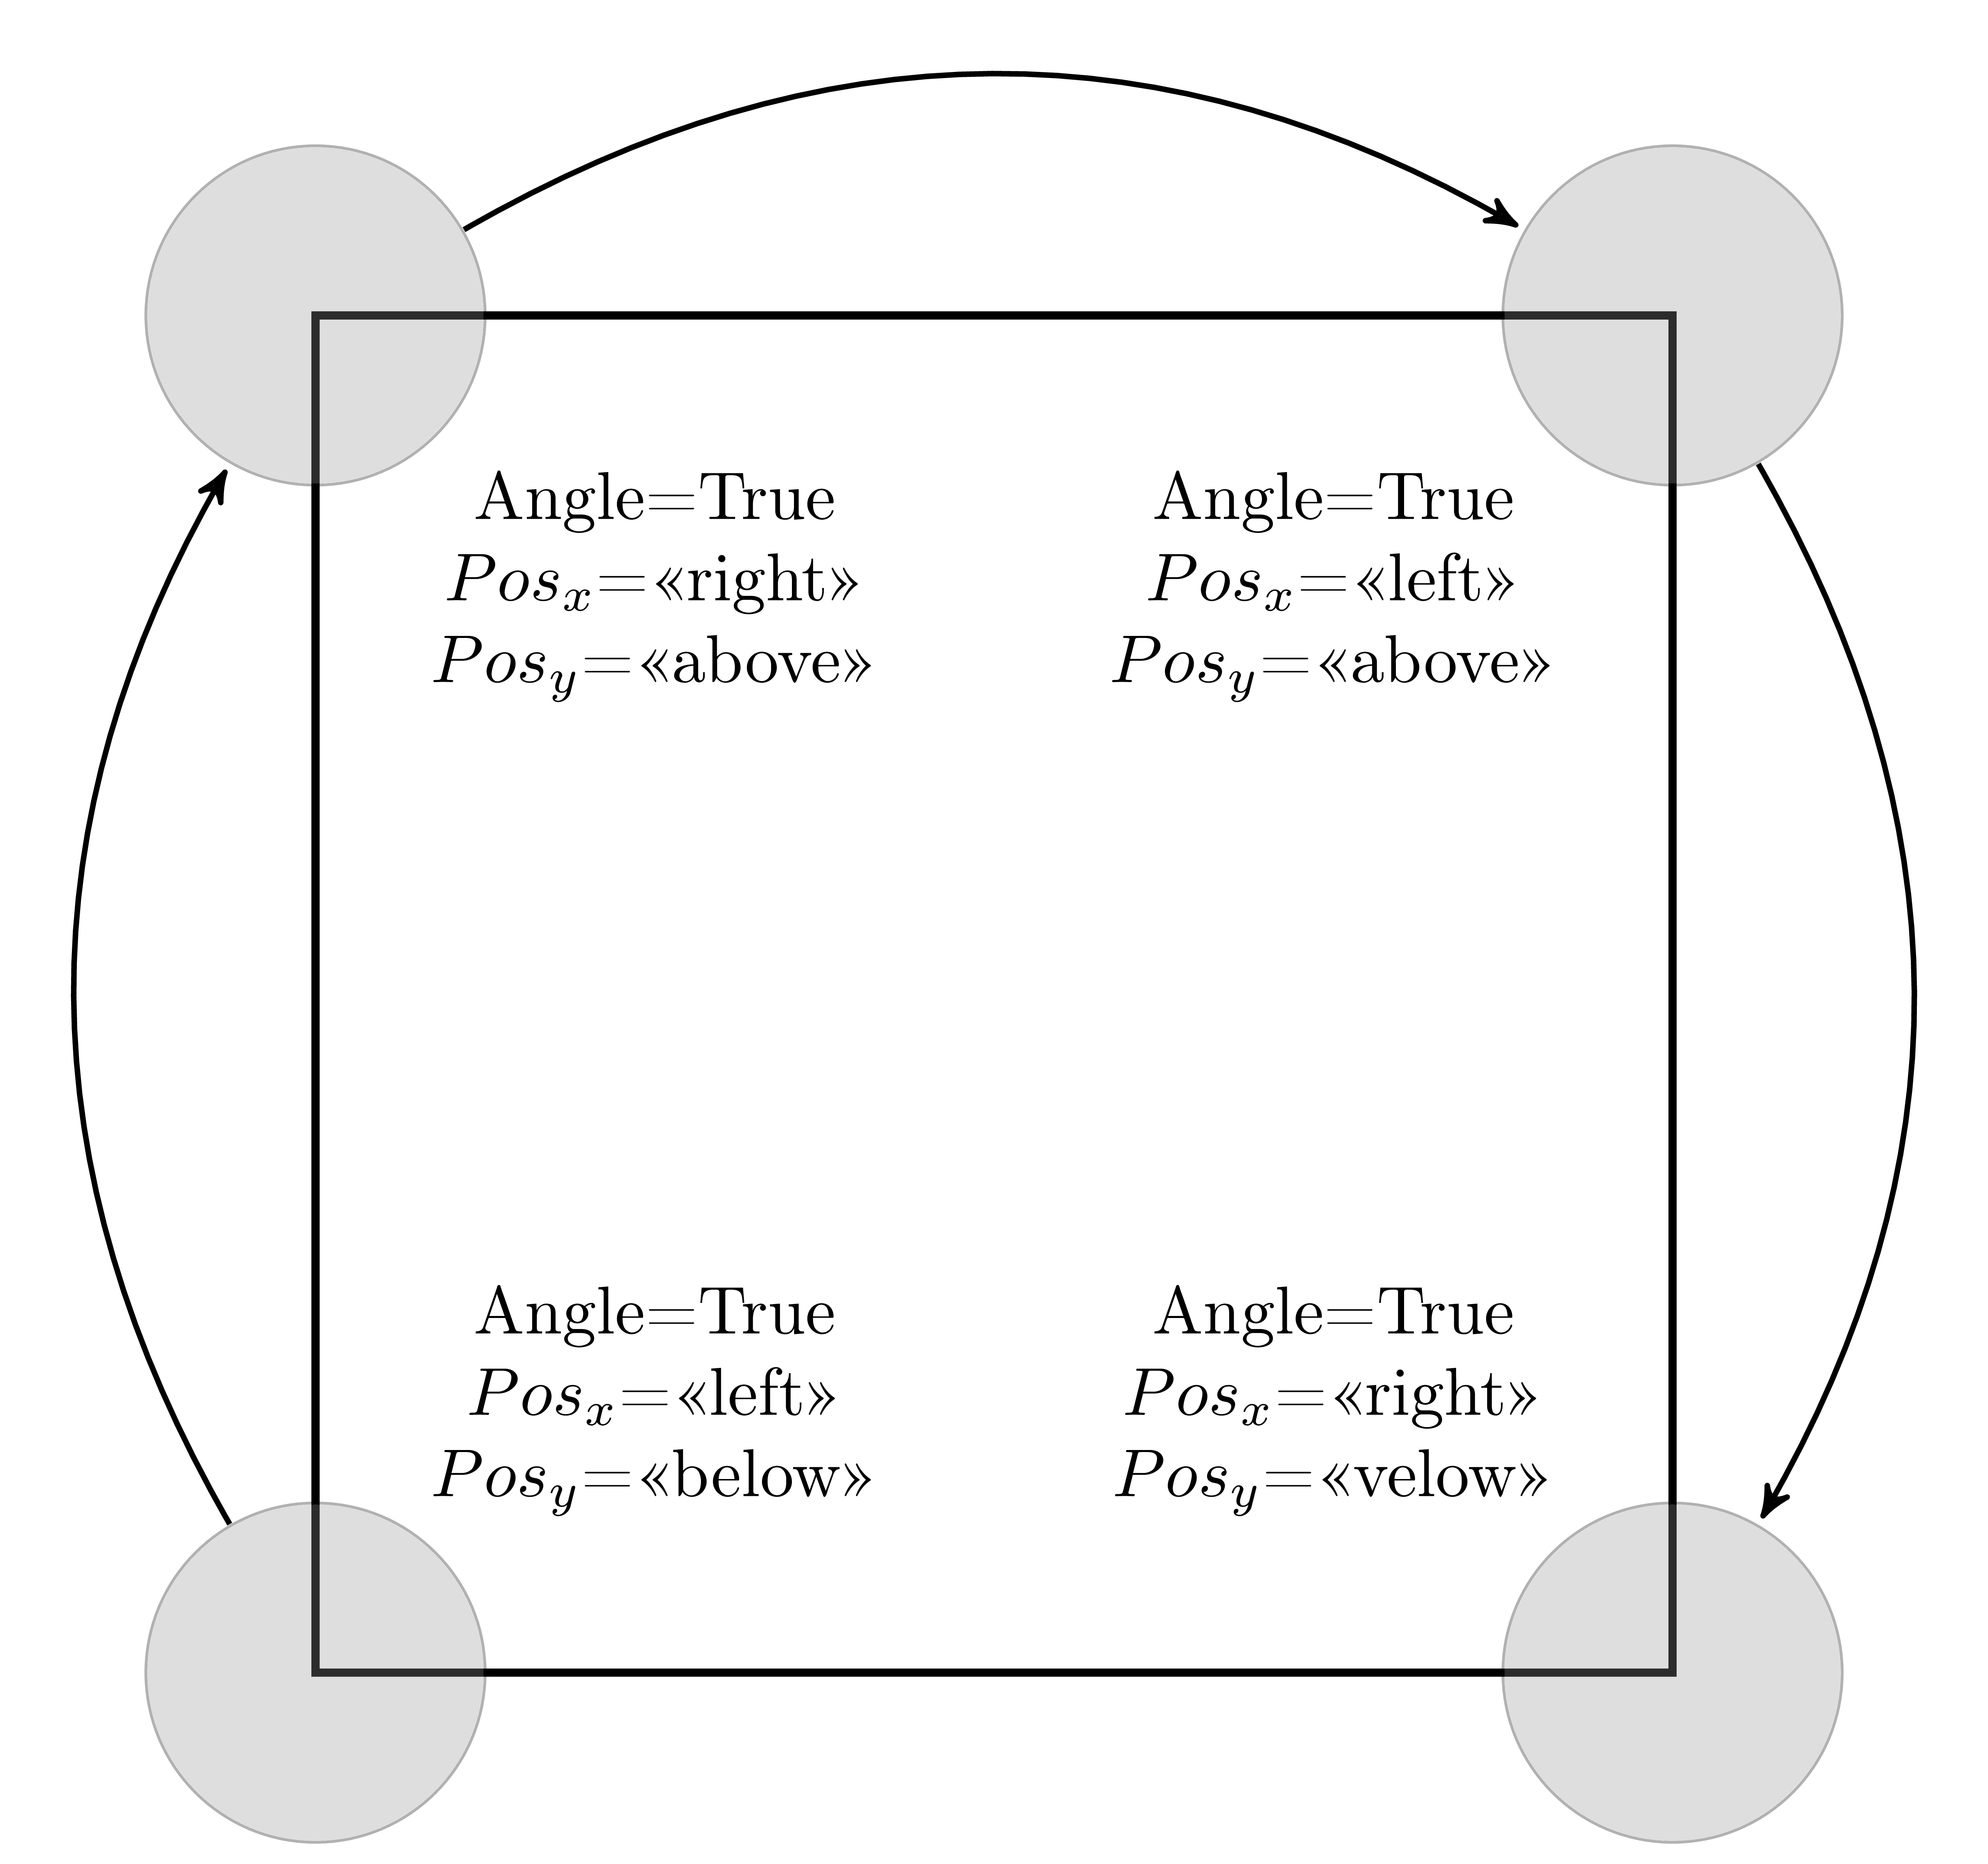
\includegraphics[width=0.7\textwidth]{square_en}
	\caption{Visual interpretation of the causal matrix}		
	\label{fig:square}
\end{figure}

Several causal matrices determining various manifestations of the represented object or process (e.g. another order of sensor triggering) may correspond to the image of each sign. We will designate the complete sequence of causal matrices of the sign $s$ image as $Z^p(s)$. 

The case, in which a sign's characteristics are data received by sensors, is a special one. In a more general statement, a sign's image attributes are other signs representing these specific characteristics. Thus, we are capable of associating the image of sign $s$ with set $S_p(s)$, having the potency of $q$. Each element of the set corresponds to the number of lines of causal matrix $z$, having the dimensions of $q$ by $h$, that is, each feature $s_i\in S_p(s)$ corresponds to an attribute bit vector setting at position 1 moments in time, when this attribute should be present in input data to actualize the sign $s$ (recognize the image of the sign). 

To refine the definition of the set $S_p(s)$, let us introduce a class of binary relations $\{\sqsubset_p,\sqsubset_p^1,\sqsubset_p^2,\dots\}$ determined by Cartesian product $S\times S$. Let us suppose that the sign $s_i$ is \textit{an image component} of sign $s$, $(s_i,s)\in\sqsubset_p$ or $s_i\sqsubset_p s$ if $s_i\in S_p(s)$. If it is known that the sign $s_i$ corresponds to 1 in $t$th column of a certain causal matrix $z\in Z^p(s)$ of sign $s$, we shall use nested relation $\sqsubset_p^t\subset \sqsubset_p$.

\subsection{Causal Network}\label{subsec:causal_net}

Let us introduce a special procedure $\Lambda_p: 2^Z\rightarrow 2^{\mathbb N}\times 2^{\mathbb N}$, which associates to every list of causal matrices $Z^p(s)\subset Z$ of the sign $s$ image two non-overlapping subsets of indexes of its own columns $I^c\subset\mathbb N, \forall i\in I^c\ i\leq h$ (indexes of condition columns) and $I^e\subset\mathbb N, \forall i\in I^e\ i\leq h$ (indexes of effect columns). $\Lambda_p(Z^p(s))=(I^c,I^e), I^c\cap I^e=\emptyset$. For example, if for a set of matrices $Z=\{((1, 0), (0, 1))\}$ procedure $\Lambda_p$ returns two sets $\{1\}$ and $\{2\}$ this means that the occurrence of the feature corresponding to the first line of the matrix causes an occurrence of the feature corresponding to the second line. In essence, the procedure $\Lambda_p$ is a function of establishing a cause-and-effect relationship at the set of input events and may be implemented by various means, including Norris algorithm, FcbO, or AddIntent (\cite{Norris1978,Krajca2010,Merwe2004}).

In the case when for matrices $Z^p(s)$ of the sign $s$ image, the set of effect columns is empty, $I^e=\emptyset$, that is, when it is impossible to unambiguously determine what events always precede others we will assume that a cause-and-effect relationship was not established and the sign mediates a certain object or situation. Otherwise, we will assume that the sign mediates a certain action or process, the result of which is coded in effect columns, and the condition is coded in condition columns. 

The following statements in respect to properties of procedure $\Lambda_p$ are valid:
\begin{itemize}
	\item $I^c\cap I^e=\emptyset$ --- a column of the causal matrix may not be simultaneously condition and effect;
	\item $|I^c\cup I^e|=h$ --- a column of the causal matrix is either a condition or an effect;
	\item $I^c\not = \emptyset$ --- among causal matrix columns there must be at least one condition column, whereas there may be no effects (in the case of object features);
	\item $\forall i\in I^e, j\in I^c\ i>j$ --- all conditions precede effects.
\end{itemize}
Taking the above into consideration, a causal matrix diagram is shown at Figure \ref{fig:caus_matr}.

\begin{figure}
	\centering
	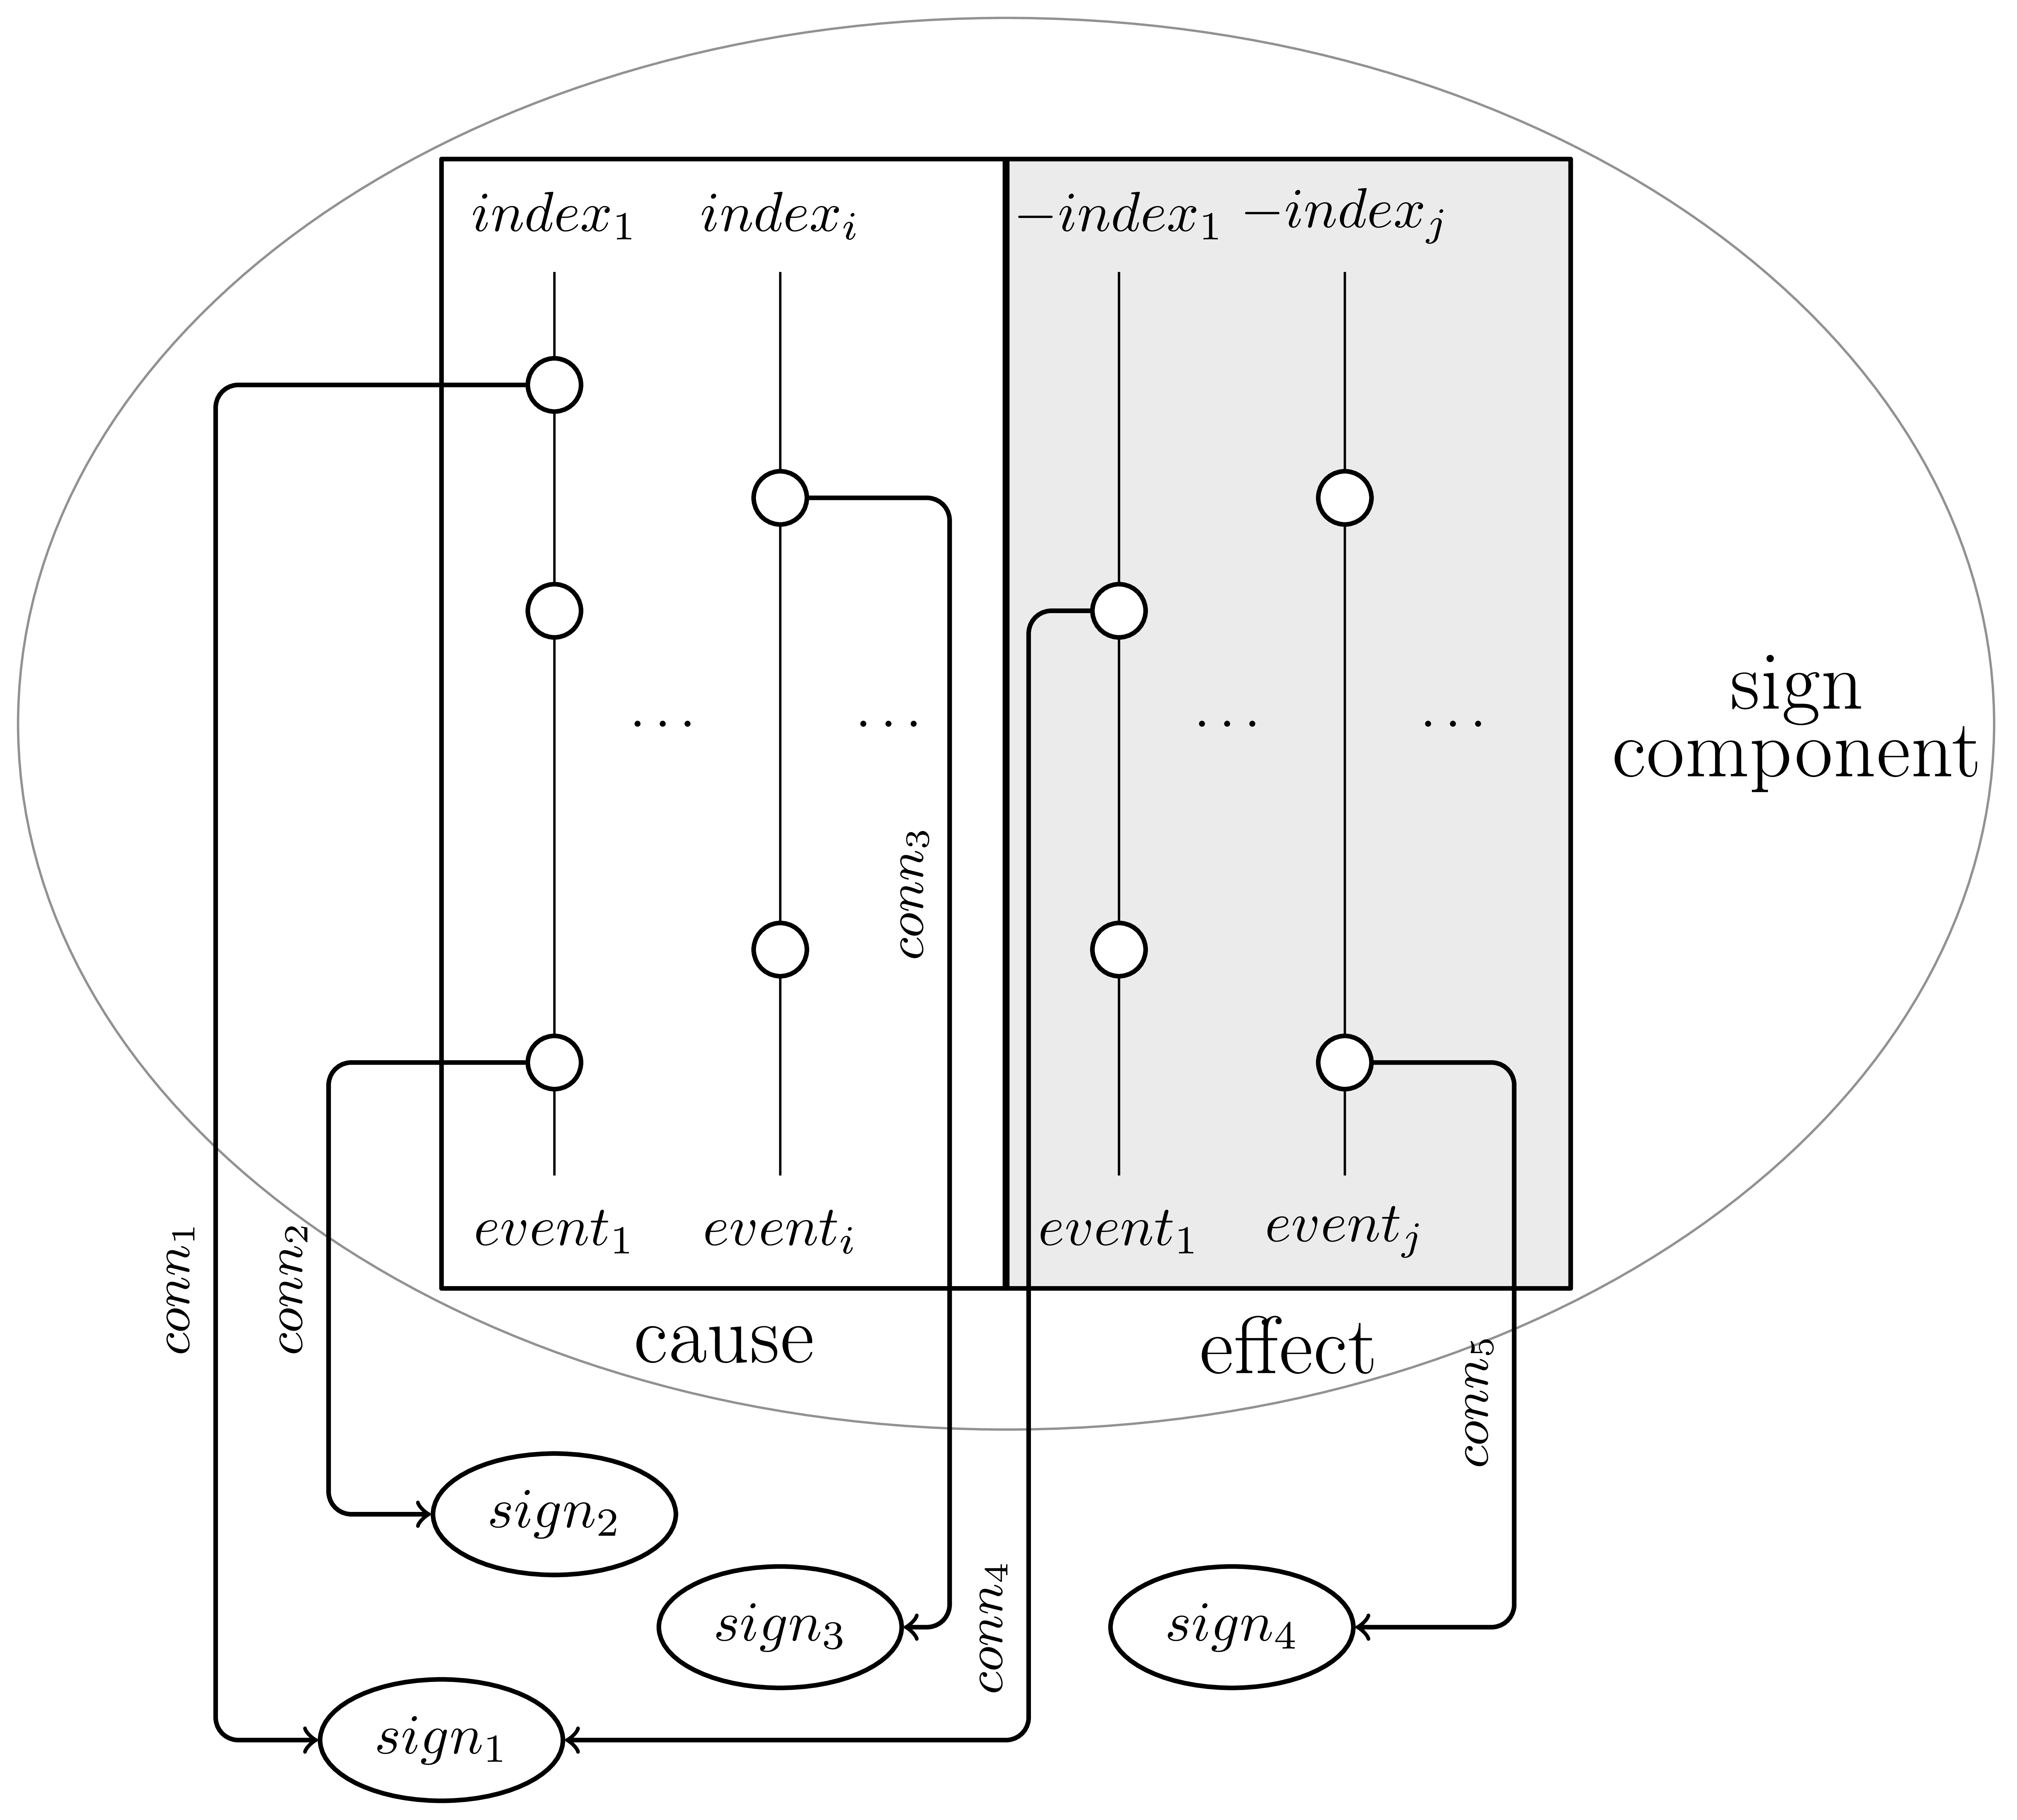
\includegraphics[width=0.7\textwidth]{caus_matr}
	\caption{Schema of the causal matrix}	
	\label{fig:caus_matr}	
\end{figure}

Let us now introduce the concept of a causal network, which will determine the heterarchy of a set of images. Causal network $W_p=\langle V_p, E_p \rangle$ is a marked orgraph in which
\begin{itemize}
	\item every node $v\in V_p$ is associated with a sequence of causal matrices $Z^p(s)$ of a certain sign $s$ image, which we will designate as $v\rightarrow Z^p(s)$;
	\item edge $e=(v_1, v_2)$ belongs to a set of graph edges $E$ if $v_1\rightarrow Z^p(s_1), v_2\rightarrow Z^p(s_2)$ and $s_1\in S_p(s_2)$, i.e. if the sign $s_1$ is an element of sign image $s_2$;
	\item each graph edge $e=(v_1, v_2), v_1\rightarrow Z^p(s_1), v_2\rightarrow Z^p(s_2)$ is associated with the label $\epsilon=(\epsilon_1,\epsilon_2,\epsilon_3)$, a tuple of three natural numbers:
	\begin{itemize}
		\item $\epsilon_1$ --- index of the initial matrix of the sequence $Z^p(s_1)$ may possess a special value of 0 if any matrices of the sequence may serve as source matrices;
		\item $\epsilon_2$is the target matrix in the sequence $Z^p(s_2)$ the line of which is associated with feature $s_1$;
		\item $\epsilon_3$ is the index of a column in the target matrix in which the value of the line corresponding to feature $s_1$ is 1, and the index may possess positive values (condition columns) or negative values (effect columns).
	\end{itemize}		
\end{itemize}

A causal network represents a certain set of overlapping hierarchies of signs. Every sign is represented by a set of causal matrices determining the image of the sign, and hierarchy represents hierarchical relations between images. This relation may be read as follows: ``sign $x$ participates in the formation of image of sign $y$''. Here we specify for what specific matrix of sign $y$ and for what specific column of this matrix sign $x$ is required (labels $\epsilon_2$ and $\epsilon_3$ accordingly). In some cases, we may also state sign matrix $x$ (label $\epsilon_1$) participating in the process. The example of such a network is shown on Figure \ref{fig:caus_net}.

\begin{figure}
	\centering
	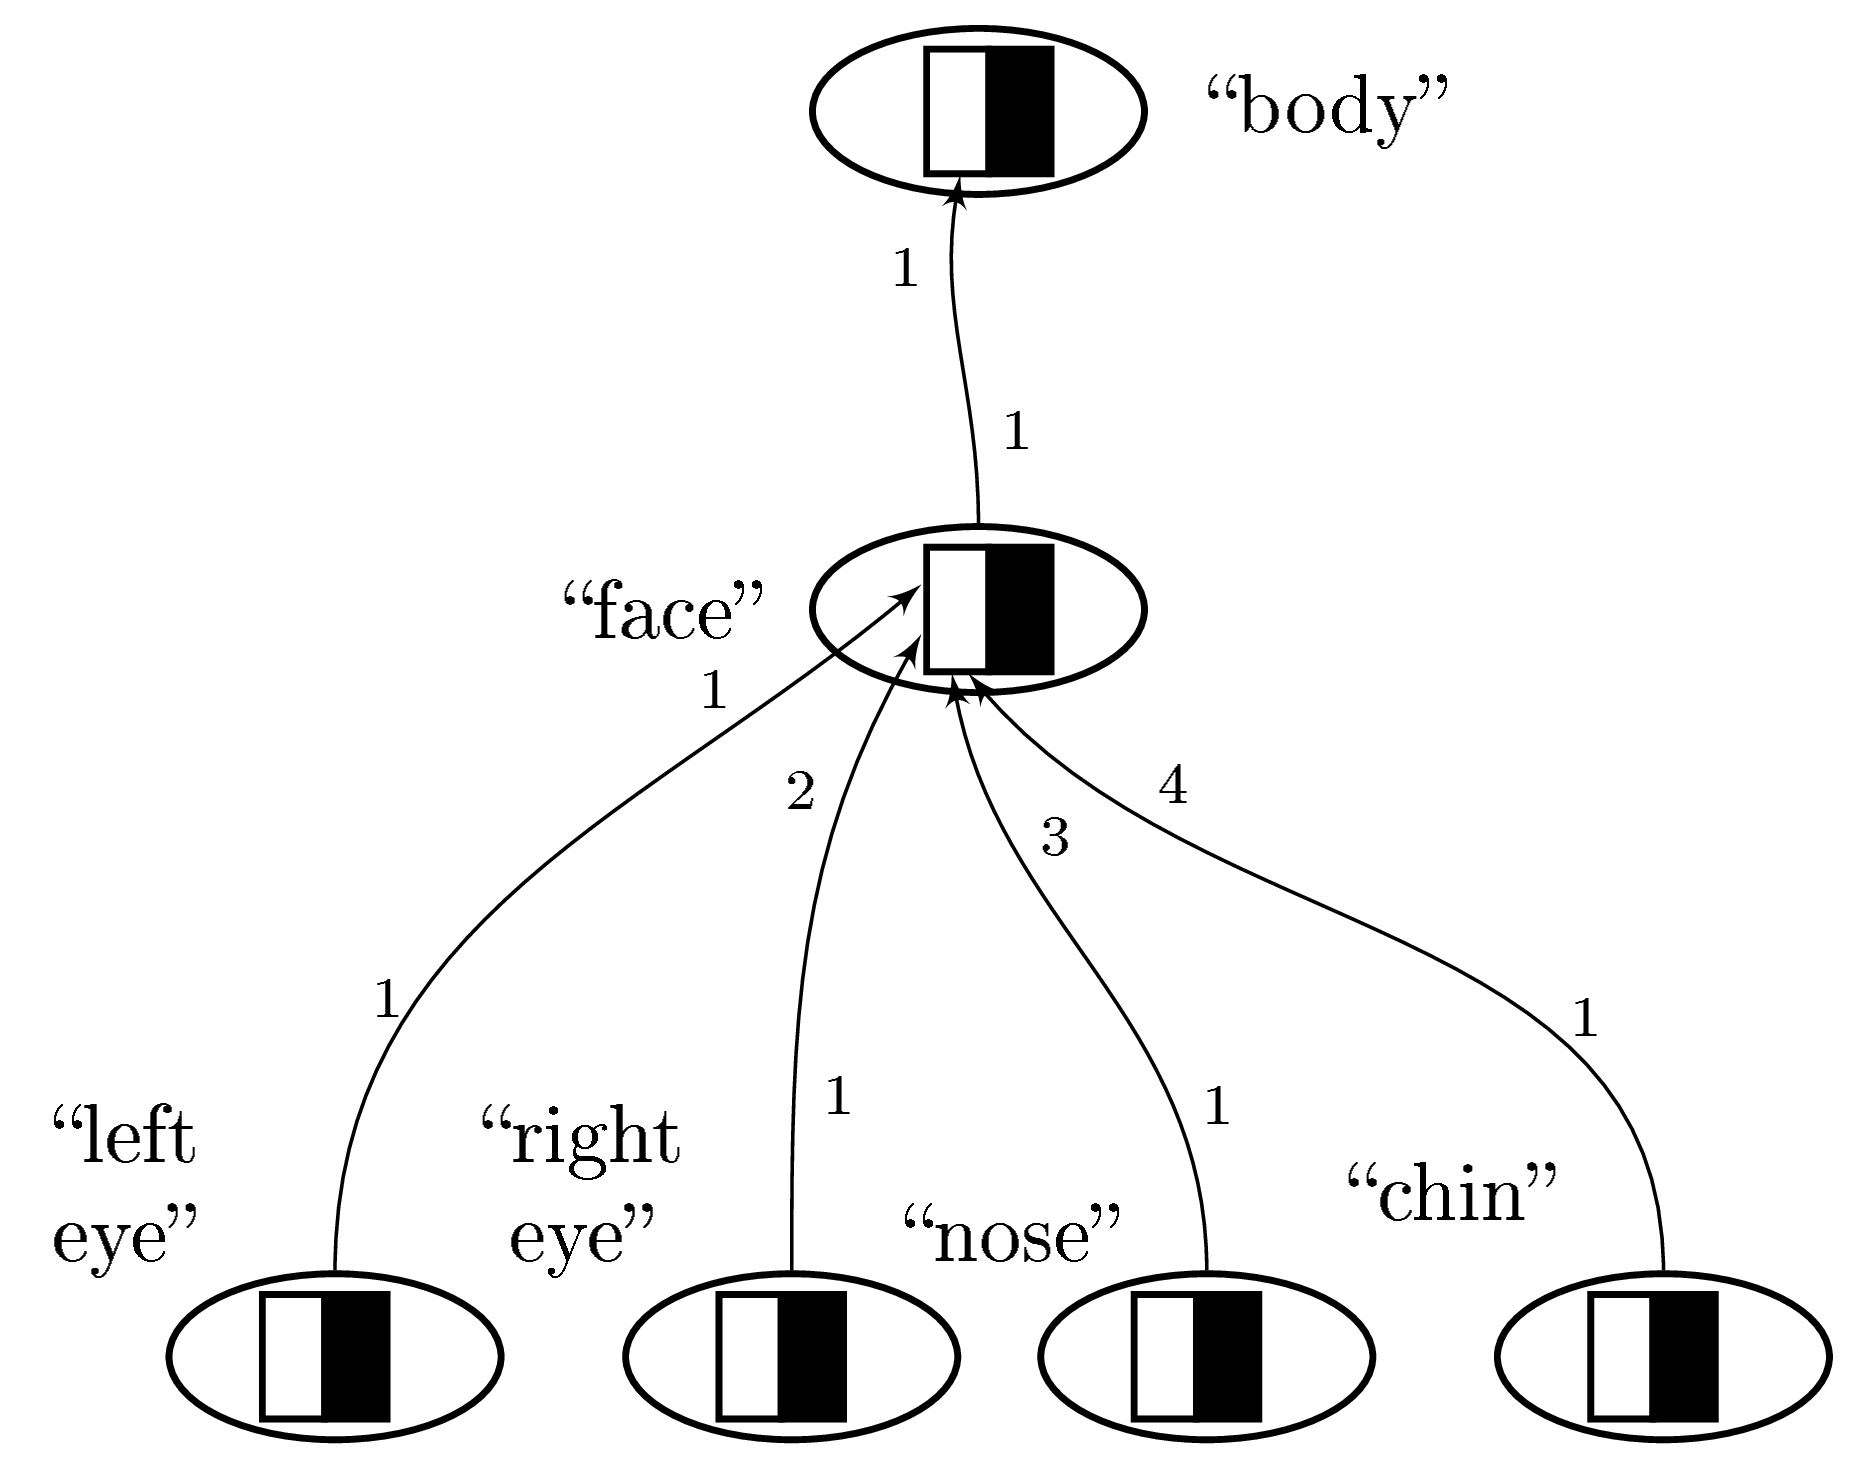
\includegraphics[width=0.7\textwidth]{caus_net_en}
	\caption{Schema of the causal network. Causal matrices are displayed as squares, condition columns are the left white part of the square,  effect columns - the right black part of the square. Label $\epsilon_1$ is placed at the beginning of each arrow, label $\epsilon_2$ is defined as square number in the oval node, label $\epsilon_3$  is placed at the end of each arrow.}
	\label{fig:caus_net}		
\end{figure}

Similarly, causal networks are determined for the remaining elements of the sign --- for significance and personal meaning. For each sign $s$, sets $S_m(s)$ and $S_a(s)$ are determined, that is, classes of relations $\{\sqsubset_m,\sqsubset_m^1,\sqsubset_m^2,\dots\}$ and $\{\sqsubset_a,\sqsubset_a^1,\sqsubset_a^2,\dots\}$ are determined. Set $S_m(s)$ is interpreted as the role composition of sign $s$, for example, a subset element or action role. Set $S_a(s)$ is interpreted as the immediate element composition of a certain situation observed and experienced presently by a subject, which is a bearer of a world model. Similarly, sets $Z^m(s)$ and $Z^a(s)$, as well as procedures $\Lambda_m$ and $\Lambda_a$ are determined.


\section{Semiotic network}\label{sec:semiotics}

Let us define sign $s$ as a quadruple $\langle n, p, m, a\rangle$ where $n$ is the name of the sign; $p$ is the image of the sign, a sequence of causal matrices $\langle z_1^p(s), z_2^p(s), \dots\rangle$ corresponding to node $w_p(s)$ of the causal matrix for images; $m$ is the significance of the sign, a sequence of causal matrices $\langle z_1^m(s), z_2^m(s), \dots\rangle$ corresponding to node $w_m(s)$ of the causal matrix for significances; and $a$ is the personal meaning of the sign, a sequence of causal matrices $\langle z_1^a(s), z_2^a(s), \dots\rangle$ corresponding to node $w_a(s)$ of the causal matrix for meanings.

Let us define \textit {semiotic network} as the quintuple $\Omega=\langle W_p, W_m, W_a, R_n, \Theta \rangle$ where
\begin{itemize}
	\item $W_p, W_m, W_a$ are causal networks within the set of images, significances and personal meanings, respectively;
	\item $R_n$ is a class of relations within the set of signs generated, based on the three causal networks, that is $R_n=\{R_p, R_m, R_a\}$;
	\item $\Theta$ is the class of operations of a set of signs, which are generated based on three types of causal networks to which respective sign elements belong (see \cite{Osipov2014c} for more detail).
\end{itemize} 

We must emphasize one more time that a sign represents not only the objects of the external world, but also the processes occurring in it, realizable actions, as well as the situations observed in the external environment. The three types of causal networks composing a semiotic network are not independent from each other. The following unambiguous correspondence is established among the nodes of each network: for each node $w_x$ of network $W_x$, such unique nodes $w_y$ and $w_z$ may be found within networks $W_y, W_z$ ($x,y,z\in\{p,m,a\}$) so that all three nodes correspond to the same sign $s=\langle w_p, w_m, w_a\rangle$. A sign's name is the label of nodes in each of the networks: in the causal network, there may be only one node with this label and nodes of all networks with the same labels compose elements of the sign. To associate causal matrices having different types of nodes within one sign, special binding functions are used: $\Psi_p^m, \Psi_m^a,\Psi_a^p$, and functions opposite to them $\Psi_m^p,\Psi_a^m,\Psi_p^a$ \cite{Osipov2014c}. Every binding function associates a causal matrix of one type with a causal matrix of another type or generates this matrix in case it is absent in the respective node of the network.

Let us introduce the concepts of activity in a semiotic network and of its propagation process. Let us introduce a label of activity for causal matrices of network $W_x$ ($x\in\{p,m,a\}$) and call matrix set $Z_x^*$, having the label ``active''. An activity propagation process is an alteration of the composition of set $Z_x^*$ over time (at each discrete moment of time) and is described for each type of causal network with the following intrinsic function: $\varphi_a, \varphi_m,\varphi_p$. An activity propagation process is iterative, i.e., at each step a new composition of active matrices is initiated based on the previous composition and it depends on the matrices included in it. In the simplest case, we will discuss the process in which each matrix does not influence the course of activity propagation from another matrix, and consequently, we will assume that functions $\varphi_x$ accept one active matrix as an input and generate a new subset of active matrices. 

Due to the fact that the edges of causal networks have directions, we will distinguish the propagation of activity upward within a network, if edges outbound from a node ($\varphi_x^\uparrow$ functions) are used, and the propagation of activity downward within a network, if edges inbound to a node ($\varphi_x^\downarrow$ functions) are used. Further, describing a planning algorithm we will need only the functions of significances and personal meaning networks. We will parametrize each function $\varphi_x^\uparrow,\varphi_x^\downarrow$ by the depth of activity propagation $d_x$, which shows at which depth edges can be viewed in a given direction (upward or downward).

Further, when describing a planning algorithm we will use the concept of causal network fragment. We will define a fragment $F$ as a certain set of nodes $V$ of network $W_x=\langle V_x,E_x\rangle$ together with all the edges $E$ connecting them: $F=\langle V,E\rangle: V\subseteq V_x$ and $\forall e=(v_1,v_2)\in E v_1\in V, v_2\in V$.


\section{Planning in Sign World Model}\label{sec:plan}

The process of planning in a sign world model is implemented with the use of the MAP algorithm and is implemented inversely - from the final to the initial situation. Let us briefly describe the main stages of the algorithm's operation. A problem definition is at the input, 
\[
	T = \langle N_T,S,Sit_{start}, Sit_{goal}\rangle,
\]
where $N_T$ is the problem identifier, $S$ is the set of signs of a semiotic network, $Sit_{start}=\langle id_{start}, \emptyset, \emptyset, a_{start} \rangle$ is the initial state having the meaning of $a_{start}=\{z_{start}^a\}$ and $Sit_{goal}=\langle id_{goal}, \emptyset, \emptyset, a_{goal} \rangle$ is the target situation $a_{goal}=\{z_{goal}^a\}$ where $z^a_i$ is the causal matrix of the corresponding personal meaning. In this case significances and images of situations are empty because we don't consider recognition and communication part of the task; we use only personal information about situations. In general, problem $T$ is the result of a ``designation'' procedure, that is, the result of forming a world model using the initial descriptions of planning domain $D$, which sets the lists of possible actions and object types, as well as planning problems $P$. The world model includes the definitions of the starting conditions and of the final goal (step \ref{alst:ground}).

The result of MAP planning is a plan. $Plan=\{\langle z_{s1}^a,z_{p1}^a\rangle, \langle z_{s2}^a,z_{p2}^a\rangle,\dots, \langle z_{sn}^a,z_{pn}^a\rangle\}$, a sequence with the length of $n$ pairs $\langle z_{si}^a,z_{pi}^a\rangle$, where $z_{si}^a$ is the causal matrix of a certain network node for personal meanings representing a $i$th planning situation, and $z_{pi}^a$ is the causal matrix of certain personal meaning representing the action used in situation $z_{si}^a$. Here, the situation $z_{si+1}^a$ is the result of the performance of action $z_{pi}^a$ in the meaning that will be elaborated further during the discussion of the algorithm, $z_{s1}^a := z_{start}^a$ is the causal matrix corresponding to the meaning of the initial situation, and $z_{sn}^a=z_{goal}^a)$ is the causal matrix corresponding to the meaning of the target situation.

\begin{algorithm}[H]
	\label{alg:plan}
	\begin{algorithmic}[1]
		\Require planning domain $D$, planning task $P$, maximal iteration deep $i_{max}$
		\Ensure plan $Plan$
		
		\vspace*{1pt}
		\hrule
		\vspace*{5pt}
		
		\State T = $\langle N_T,S,Sit_{start}, Sit_{goal}\rangle$ := \Call{ground}{$P$}\label{alst:ground}
		
		\Statex\Comment{$N_T$ - task id, $S$ - set of signs, $Sit_{start}=\langle id_{start} \emptyset, \emptyset, \{z_{start}^a\} \rangle$ - start situation with meaning $a_{start}$, $Sit_{goal}=\langle id_{goal} \emptyset, \emptyset, \{z_{goal}^a\} \rangle$ - goal situation with meaning $a_{goal}$}
		\State $Plan$ := \Call{map\_search}{$T$}
		
		
		\Function{map\_search}{$T$}
		\State $z_{cur} := z_{goal}^a$
		\State $z_{start} := z_{start}^a$
		\State $Plans$ := \Call{map\_iteration}{$z_{cur}$,$z_{start}$, $\emptyset$, 0}\label{alst:start_iter}
		\State $\{Plan_0, Plan_1,\dots\}$ = \Call{sort}{$Plans$}\label{alst:sort}
		\State\Return $Plan_0$\label{alst:return}
		\EndFunction
		\algstore{algst:store1}
	\end{algorithmic}
\end{algorithm}

The planning process is hierarchical and consists in the repetition of MAP iterations, including four stages (see Figure \ref{fig:plan_algo}):
\begin{itemize}
	\item \textit{S-stage} is the search for a precedent for performing actions in the current situation;
	\item \textit{M-stage} is the search for applicable actions in the network of significances;
	\item \textit{A-stage} is the generation of personal meanings, which correspond to the significances found;
	\item \textit{P-stage} is the building of a new situation using the feature set of conditions for the actions found.
\end{itemize}

\begin{figure}
	\centering
	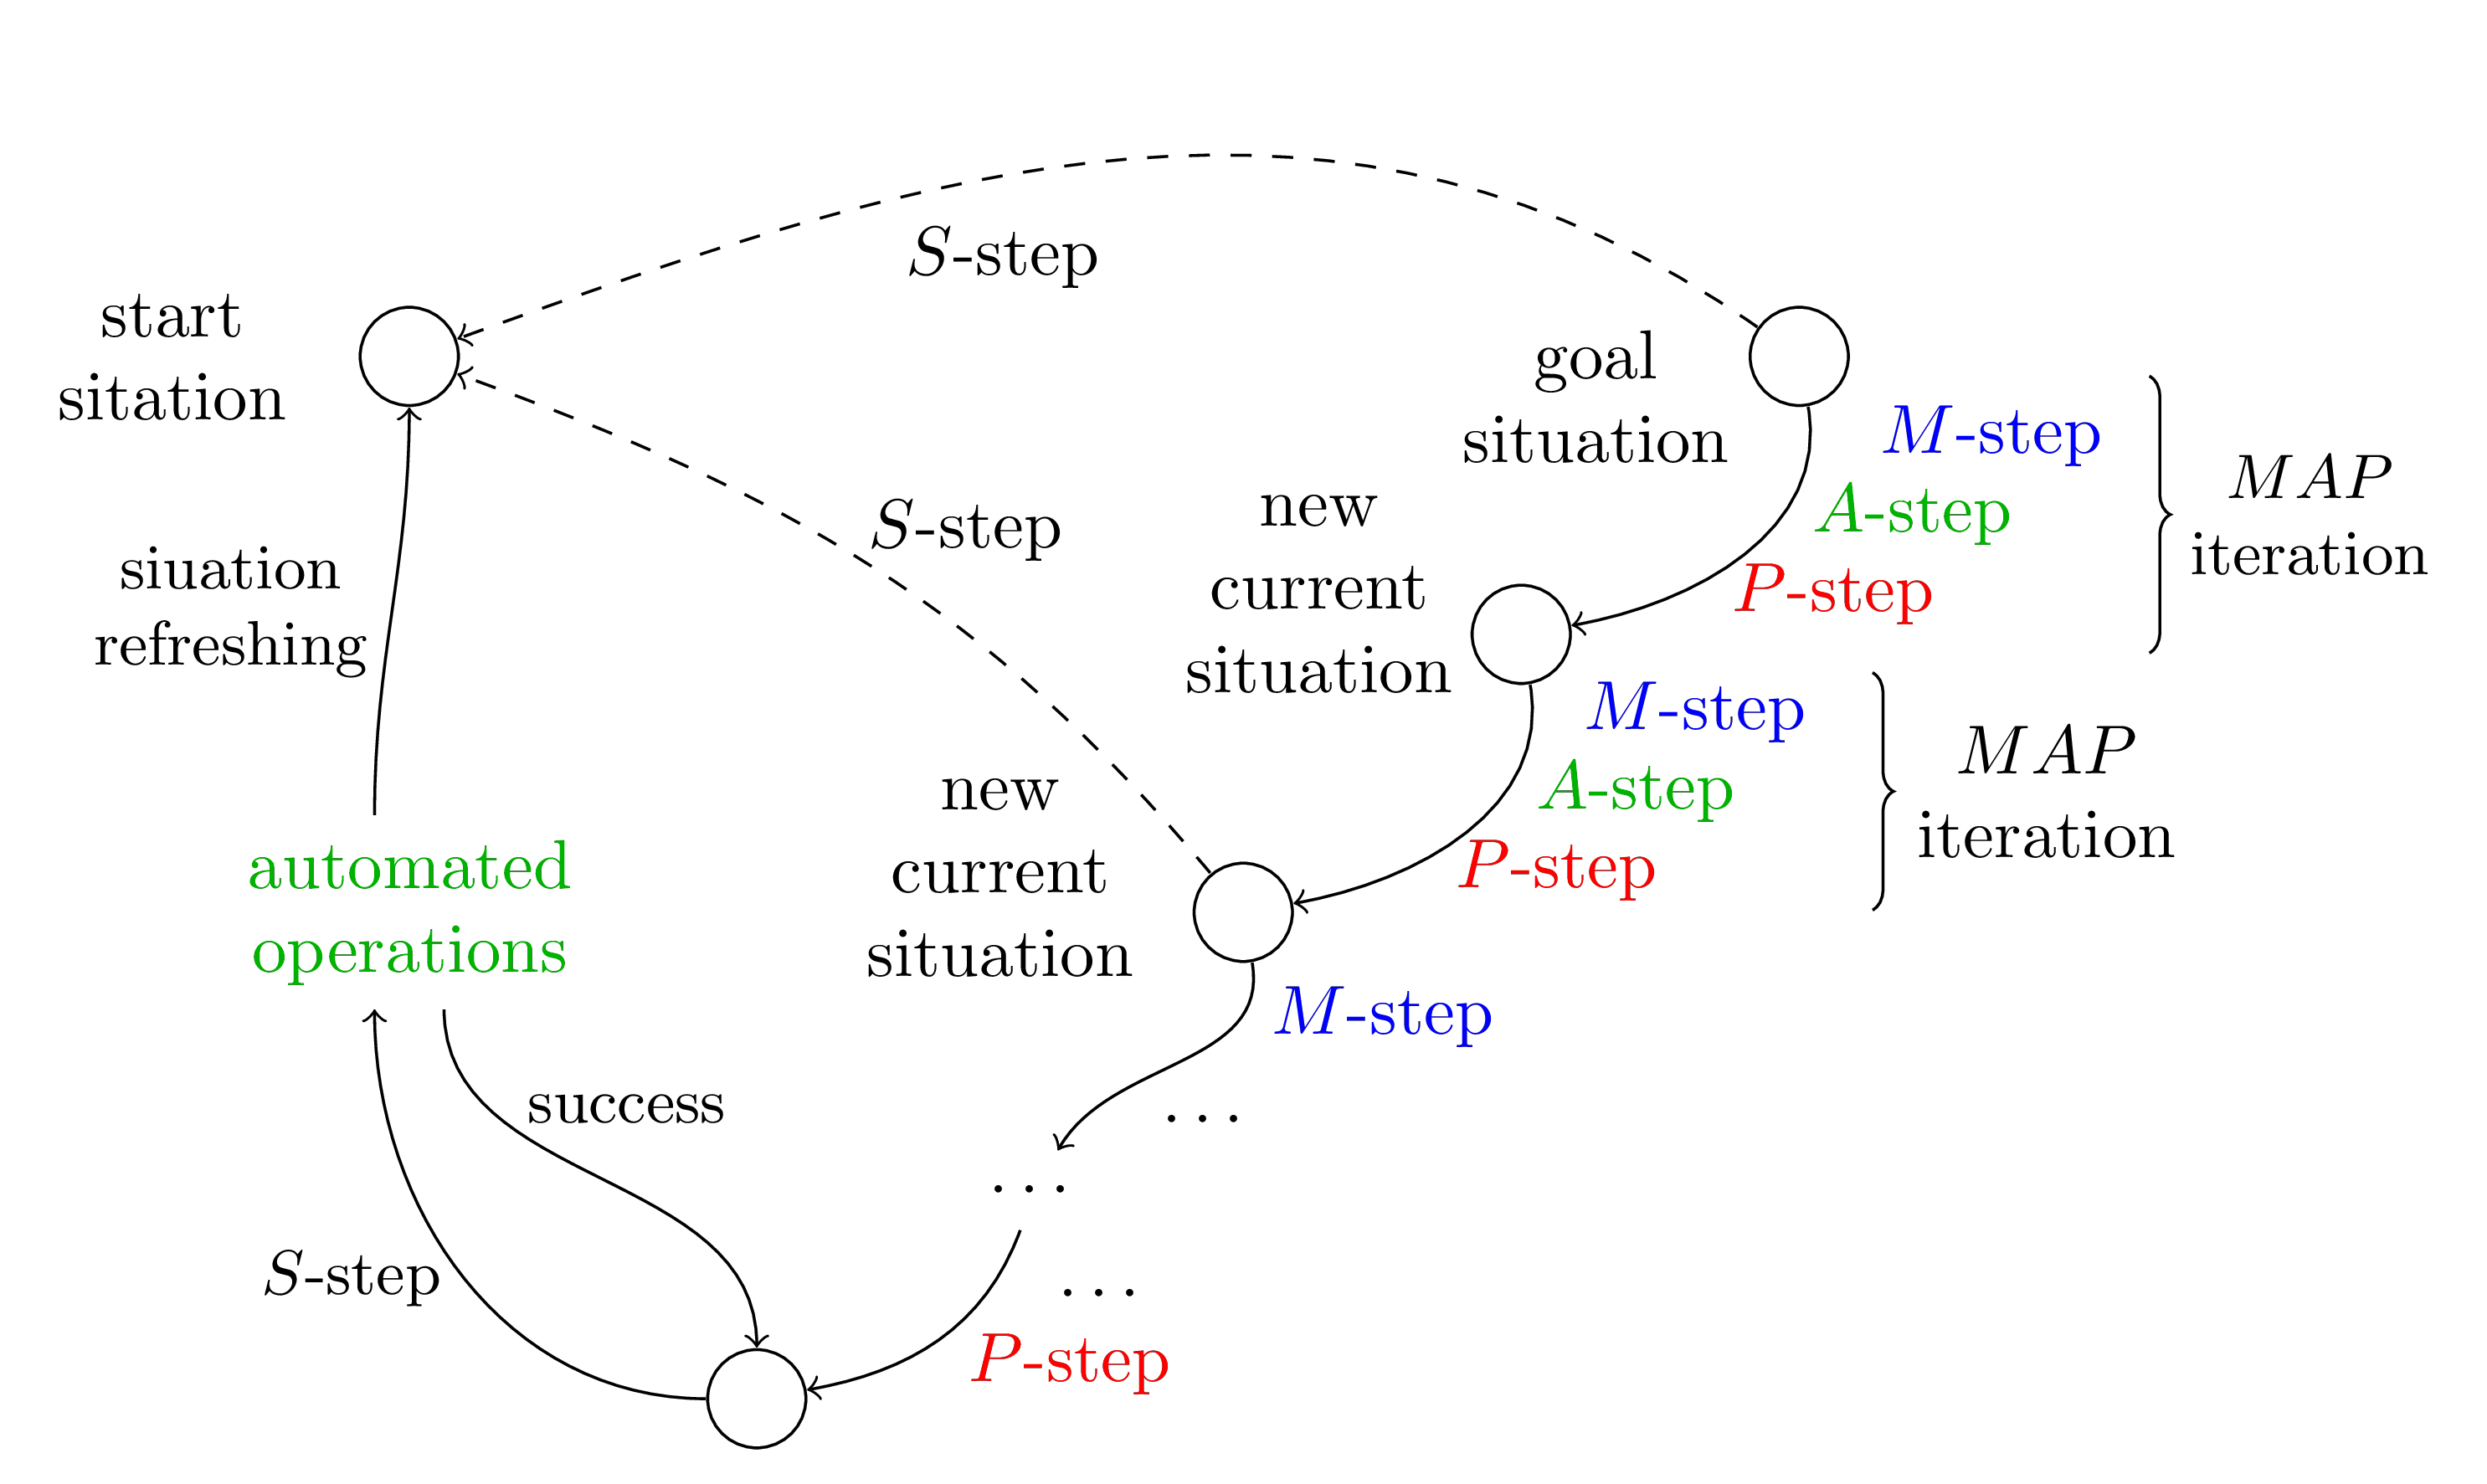
\includegraphics[width=\textwidth]{beh_plan2_en}
	\caption{Schema of the behavior planning process}	
	\label{fig:plan_algo}	
\end{figure}

In brief, MAP algorithm performs an iterative generation of causal matrices $z_{next}$ of personal meanings based on the current active matrix $z_{cur}$ until the maximum number of steps $i_{max}$ is reached (step \ref{alst:exit}), or the initial matrix $z_{start}$ (step \ref{alst:suc_exit}) corresponding to the personal meaning $a_{start}$ of the initial situation is completely activated. A matrix corresponding to the personal meaning of target situation $z_{goal}^a$ (step \ref{alst:start_iter}) serves as an active causal matrix for the first iteration. Upon completion of all iterations, the plans found are sorted by length (step \ref{alst:sort}), and the shortest of them represent the solution of the planning problem in the sign world model (step \ref{alst:return}).

The first stage of MAP iteration is S-stage. Its essence is that the search for precedents is performed within the world model of an intelligent agent, i.e., a search for actions that were performed in current conditions $z_{cur}$. To achieve that, all signs in world model $S$ are reviewed, as well as their personal meanings $a(s)$ (steps\ref{alst:check_wm} -- \ref{alst:check_a}). If current conditions $z_{cur}$ are satisfied with matrix $z_a$, the list of precedents $\hat A_{case}$ is supplemented by the activity in the personal meaning networks of sign $s$ for the distance of $d_a$ (step \ref{alst:search_case}).

\begin{algorithm}
	\begin{algorithmic}[1]
		\algrestore{algst:store1}
		\Function{map\_iteration}{$z_{cur}$,$z_{start}$, $Plan_{cur}$, $i$}
			\If{$i \geq i_{max}$}\label{alst:exit}
			\State\Return $\emptyset$
			\EndIf
			
			\State $\hat A_{case}:=\emptyset$ \Comment{List of precedents}
			
			\Statex\Comment{$S$-stage}
			\Statex\Comment{Search of action cases for current conditions}
			
			\ForAll{$s\in S$} \label{alst:check_wm}
			\ForAll{$z_a\in a(s)$}\label{alst:check_a}
			\If{$z_a \geq z_{cur}$}
			\State $\hat A_{case} = \hat A_{case} \cup \varphi_a^\uparrow(s,d_a)$ \label{alst:search_case}
			\EndIf
			\EndFor
			\EndFor
		\algstore{algst:store2}
	\end{algorithmic}
\end{algorithm}

After that, MAP algorithm switches to M-stage, at which the propagation of activity through personal meaning is performed over the distance of $d_a$ for the purpose of activating all signs related to the current situation (step \ref{alst:state_def}). The components of the obtained set of causal matrices $A^*$ serve as the starting points for activity propagation over the network of significances: using binding function $z_a$, for each matrix $\Psi_a^m$, the required node is determined in the causal network of significances, from which activity propagates over the distance of $d_m$ (step \ref{alst:search_act}). If the activated matrices are causal, they are added to the set of active significances $M^*$ (step \ref{alst:add_signif}).

\begin{algorithm}
	\begin{algorithmic}[1]
		\algrestore{algst:store2}
		\Statex\Comment{$M$-stage}
		\Statex\Comment{Spreading of activity downward in the personal meaning network}
		\State $A^* = \varphi_a^\downarrow(z_{cur}, d_a)$\label{alst:state_def}
		\State $M^*=\emptyset$
		\ForAll{$z_a\in A^*$}
		\Statex\Comment{Spreading of activity upward in the significance network}
		\ForAll{$z_m\in \varphi_m^\uparrow(s(z_a), d_m)$} \label{alst:search_act}
		\If{$I^e(z_m) \not= \emptyset$}
		\State $M^* := M^*\cup\{z_m\}$ \label{alst:add_signif}
		\EndIf
		\EndFor
		\EndFor
		\algstore{algst:store3}
	\end{algorithmic}
\end{algorithm}

Next, we switch to A-stage, at which a causal matrix generation is performed in the personal meaning network, the former representing actions $z_{cur}$ specified in relation to current conditions determined by the active significances of the set $M^*$. For this purpose, steps \ref{alst:a_spread_m} --\ref{alst:a_gen_a} are performed, during which the propagation of activity in the causal network of significances over the distance of $d_m$ leads to the activation of a set of significances $M^*$ of signs related to role structure of procedure matrix $z_m$. After that, using binding function $\Psi_m^a$, a new causal matrix is generated in personal meaning network copying values $z_m^*$, replacing abstract signs-roles with object signs associated with roles by a set-subset relation. Further, at A-stage, selection of causal matrices is performed that represent the actions  in current conditions $z_{cur}$ (steps \ref{alst:a_shift} -- \ref{alst:a_filter}) is performed. For this purpose, all causal matrices, the effects of which are not included in the current situation, are deleted (it should be borne in mind that planning is performed inversely). Finally, at A-stage, one of the operations within world model $\theta_a$ is performed, which provides, in this case, meta-adjustment --- checking for a certain heuristic rule, which may mean, for example, that no action may be repeated, or that it is better to perform the action that advances fastest to the initial conditions $z_{start}$ (step \ref{alst:a_meta}). Any heuristic rule can also be represented by a causal matrix of the sign's personal meaning representing the internal strategy of its behavior planning.

\begin{algorithm}
	\begin{algorithmic}[1]
		\algrestore{algst:store3}
		\Statex\Comment{$A$-stage}
		\State $\hat A_{gen}=\emptyset$
		\ForAll{$z_m\in M^*$}
		\Statex\Comment{Spreading activity downward in the significance network}
		\State $M^*=\varphi_m^\downarrow(z_m, d_m)$\label{alst:a_spread_m}
		\ForAll{$z_m^*\in M^*$}
		\State $\hat A_{gen} := \hat A_{gen}\cup\{\Psi_m^a(z_m^*)\}$ \label{alst:a_gen_a}
		\EndFor
		\EndFor
		\Statex\Comment{Merging of activity of formed meanings and meaning of the current situation}
		\State $\hat A = \hat A_{gen}\cup \hat A_{case}$
		\ForAll{$z_a\in \hat A$}
		\State $z_{shift}=(e_i|i\in I^e)$ \label{alst:a_shift}
		\If{$z_{cur} \not\geq z_{shift}$}
		\State $\hat A = \hat A\setminus\{z_a\}$ \label{alst:a_filter}
		\EndIf
		\EndFor
		\Statex\Comment{Checking of metacognitive heuristic}
		\State $\hat A=\{\theta_a(z_a)|z_a\in\hat A\}$ \label{alst:a_meta}
		\If{$\hat A = \emptyset$}
		\State\Return $\emptyset$
		\EndIf
		\algstore{algst:store4}
	\end{algorithmic}
\end{algorithm}

MAP algorithm concludes with P-stage. Here, for every generated causal matrix $z_a$, which represents a certain action, new situation $Sit_{next}$ is generated, which is the result of reverse application of action in the current conditions $z_{cur}$. Reverse application (step \ref{alst:p_next_gen}) includes the generation of a causal matrix $z_{next}$ consisting of events, which are condition columns of action $e_i\in\{e_k|e_k\in z_a, k\in I^c(z_a)$ or which belong to the current active causal matrix and are not condition columns of action $e_i\in z_{cur} \land e_i\not\in\{e_j|e_j\in z_a, j\in I^e(z_a)\}$. In the current plan $Plan_{cur}$, current conditions are applicable to action pair $\langle z_{cur}, z_a\rangle$. If the new situation does not overlap the starting situation (step \ref{alst:suc_exit}), iterations continue with the new current situation thus supplementing all sets of generated plans $Plans_{fin}$.

Constants $d_a, d_m$, which determine the depth of activity propagation within causal networks, are parameters of the algorithm and determine internal characteristics of the world model bearer, varying from agent to agent. Usually, in model experiments these parameters do not exceed 5. 

\begin{algorithm}
	\begin{algorithmic}[1]
		\algrestore{algst:store4}
			\Statex\Comment{$P$-stage}
			\State $Plans_{fin} := \emptyset$
			\ForAll{$z_a\in\hat A$}
			\State $Plan_{cur} = Plan_{cur}\cup\{\langle z_{cur}, z_a\rangle\}$
			\Statex\Comment{Generation of new situation - action application} 		
			\State $z_{next} := (e_i|(e_i\in z_{cur} \land e_i\not\in\{e_j|e_j\in z_a, j\in I^e(z_a)\}) \lor e_i\in\{e_k|e_k\in z_a, k\in I^c(z_a)\})$\label{alst:p_next_gen}
			\State $Sit_{next} = \langle id_{next}, \emptyset, \emptyset, \{z_{next}\} \rangle$
			\If{$z_{next} \geq z_{start}$}\label{alst:suc_exit}
			\State $Plans_{fin} = Plans_{fin}\cup\{Plan_{cur}\}$
			\Else
			\State $Plans_{rec}$ := \Call{map\_iteration}{$z_{next}$,$z_{start}$, $Plan_{cur}$, $i+1$}
			\State $Plans_{fin} = Plans_{fin}\cup Plans_{rec}$
			\EndIf
			\EndFor
			
			\State\Return $Plans_{fin}$
			\EndFunction
	\end{algorithmic}
\end{algorithm}

\section{A Model Experiment: Cube World}\label{sec:example}

Let us demonstrate the work of the presented behavior planning algorithm by a model experiment in which the planning domain is a ``block world'' example, well known in the field of automation planning \cite{Gupta1992}. The description of the domain in PDDL language \cite{Gerevini2009} consists of type definition of (\textit{blocks}), four predicates (\textit{ontable}, \textit{clear}, \textit{handempty}, \textit{holding}) and four actions (\textit{pick-up}, \textit{put-down}, \textit{stack}, \textit{unstack}) (see Table \ref{tab:domain}).

	\begin{table}
	\footnotesize
	\centering
	\begin{tabular}{|p{0.3\textwidth}|p{0.3\textwidth}|p{0.3\textwidth}|}
		\hline
		(define (\textbf{domain BLOCKS})
		
		(:requirements :strips :typing)
		
		(:types block)
		
		(:predicates (on ?x - block ?y - block)
		
		(ontable ?x - block)
		
		(clear ?x - block)
		
		(handempty)
		
		(holding ?x - block)
		)
		&
		(:\textbf{action pick-up}
		
		:parameters (?x - block)
		
		:precondition (and (clear ?x) (ontable ?x) (handempty))
		
		:effect
		
		(and (not (ontable ?x))
		
		(not (clear ?x))
		
		(not (handempty))
		
		(holding ?x)))
		&
		(:\textbf{action put-down}
		
		:parameters (?x - block)
		
		:precondition (holding ?x)
		
		:effect
		
		(and (not (holding ?x))
		
		(clear ?x)
		
		(handempty)
		
		(ontable ?x)))
		\\
		\hline
		(:\textbf{action stack}
		
		:parameters (?x - block ?y - block)
		
		:precondition (and (holding ?x) (clear ?y))
		
		:effect
		
		(and (not (holding ?x))
		
		(not (clear ?y))
		
		(clear ?x)
		
		(handempty)
		
		(on ?x ?y)))
		&
		(:\textbf{action unstack}
		
		:parameters (?x - block ?y - block)
		
		:precondition (and (on ?x ?y) (clear ?x) (handempty))
		
		:effect
		
		(and (holding ?x)
		
		(clear ?y)
		
		(not (clear ?x))
		
		(not (handempty))
		
		(not (on ?x ?y)))))
		&
		(define (\textbf{problem BLOCKS-4-0})
		
		(:domain BLOCKS)
		
		(:objects D B A C - block)
		
		(:INIT (CLEAR C) (CLEAR A) (CLEAR B) (CLEAR D) (ONTABLE C) (ONTABLE A)
		
		(ONTABLE B) (ONTABLE D) (HANDEMPTY))
		
		(:goal (AND (ON D C) (ON C B) (ON B A)))
		)\\
		\hline
	\end{tabular}
	\caption{Description of the planning domain ``block world'' and a task of tower building (``BLOCKS-4-0'').}
	\label{tab:domain}
\end{table}

Using MAP algorithm, let us make an example of a solution to a planning problem --- building a tower of four blocks, which lie on the table (Table \ref{tab:domain}). A fragment of causal network of personal meanings, which determines the causal matrix of meaning named \textit{start} is shown at Figure \ref{fig:start_sit}. Each separate block (\textit{a}, \textit{b}, \textit{c}, \textit{d}) has one causal matrix situated in a network node, whereas each of the predicates \textit{clear} and \textit{ontable} have four matrices in a node, since they participate in events with different blocks. For example, matrices of sign \textit{clear} are preset in the 1st, 3rd, 5th and 7th columns of the sign matrix \textit{start} simultaneously, with blocks \textit{a}, \textit{b}, \textit{c} and \textit{d} respectively, which means that no blocks are located on any of the blocks.

\begin{figure}
	\centering
	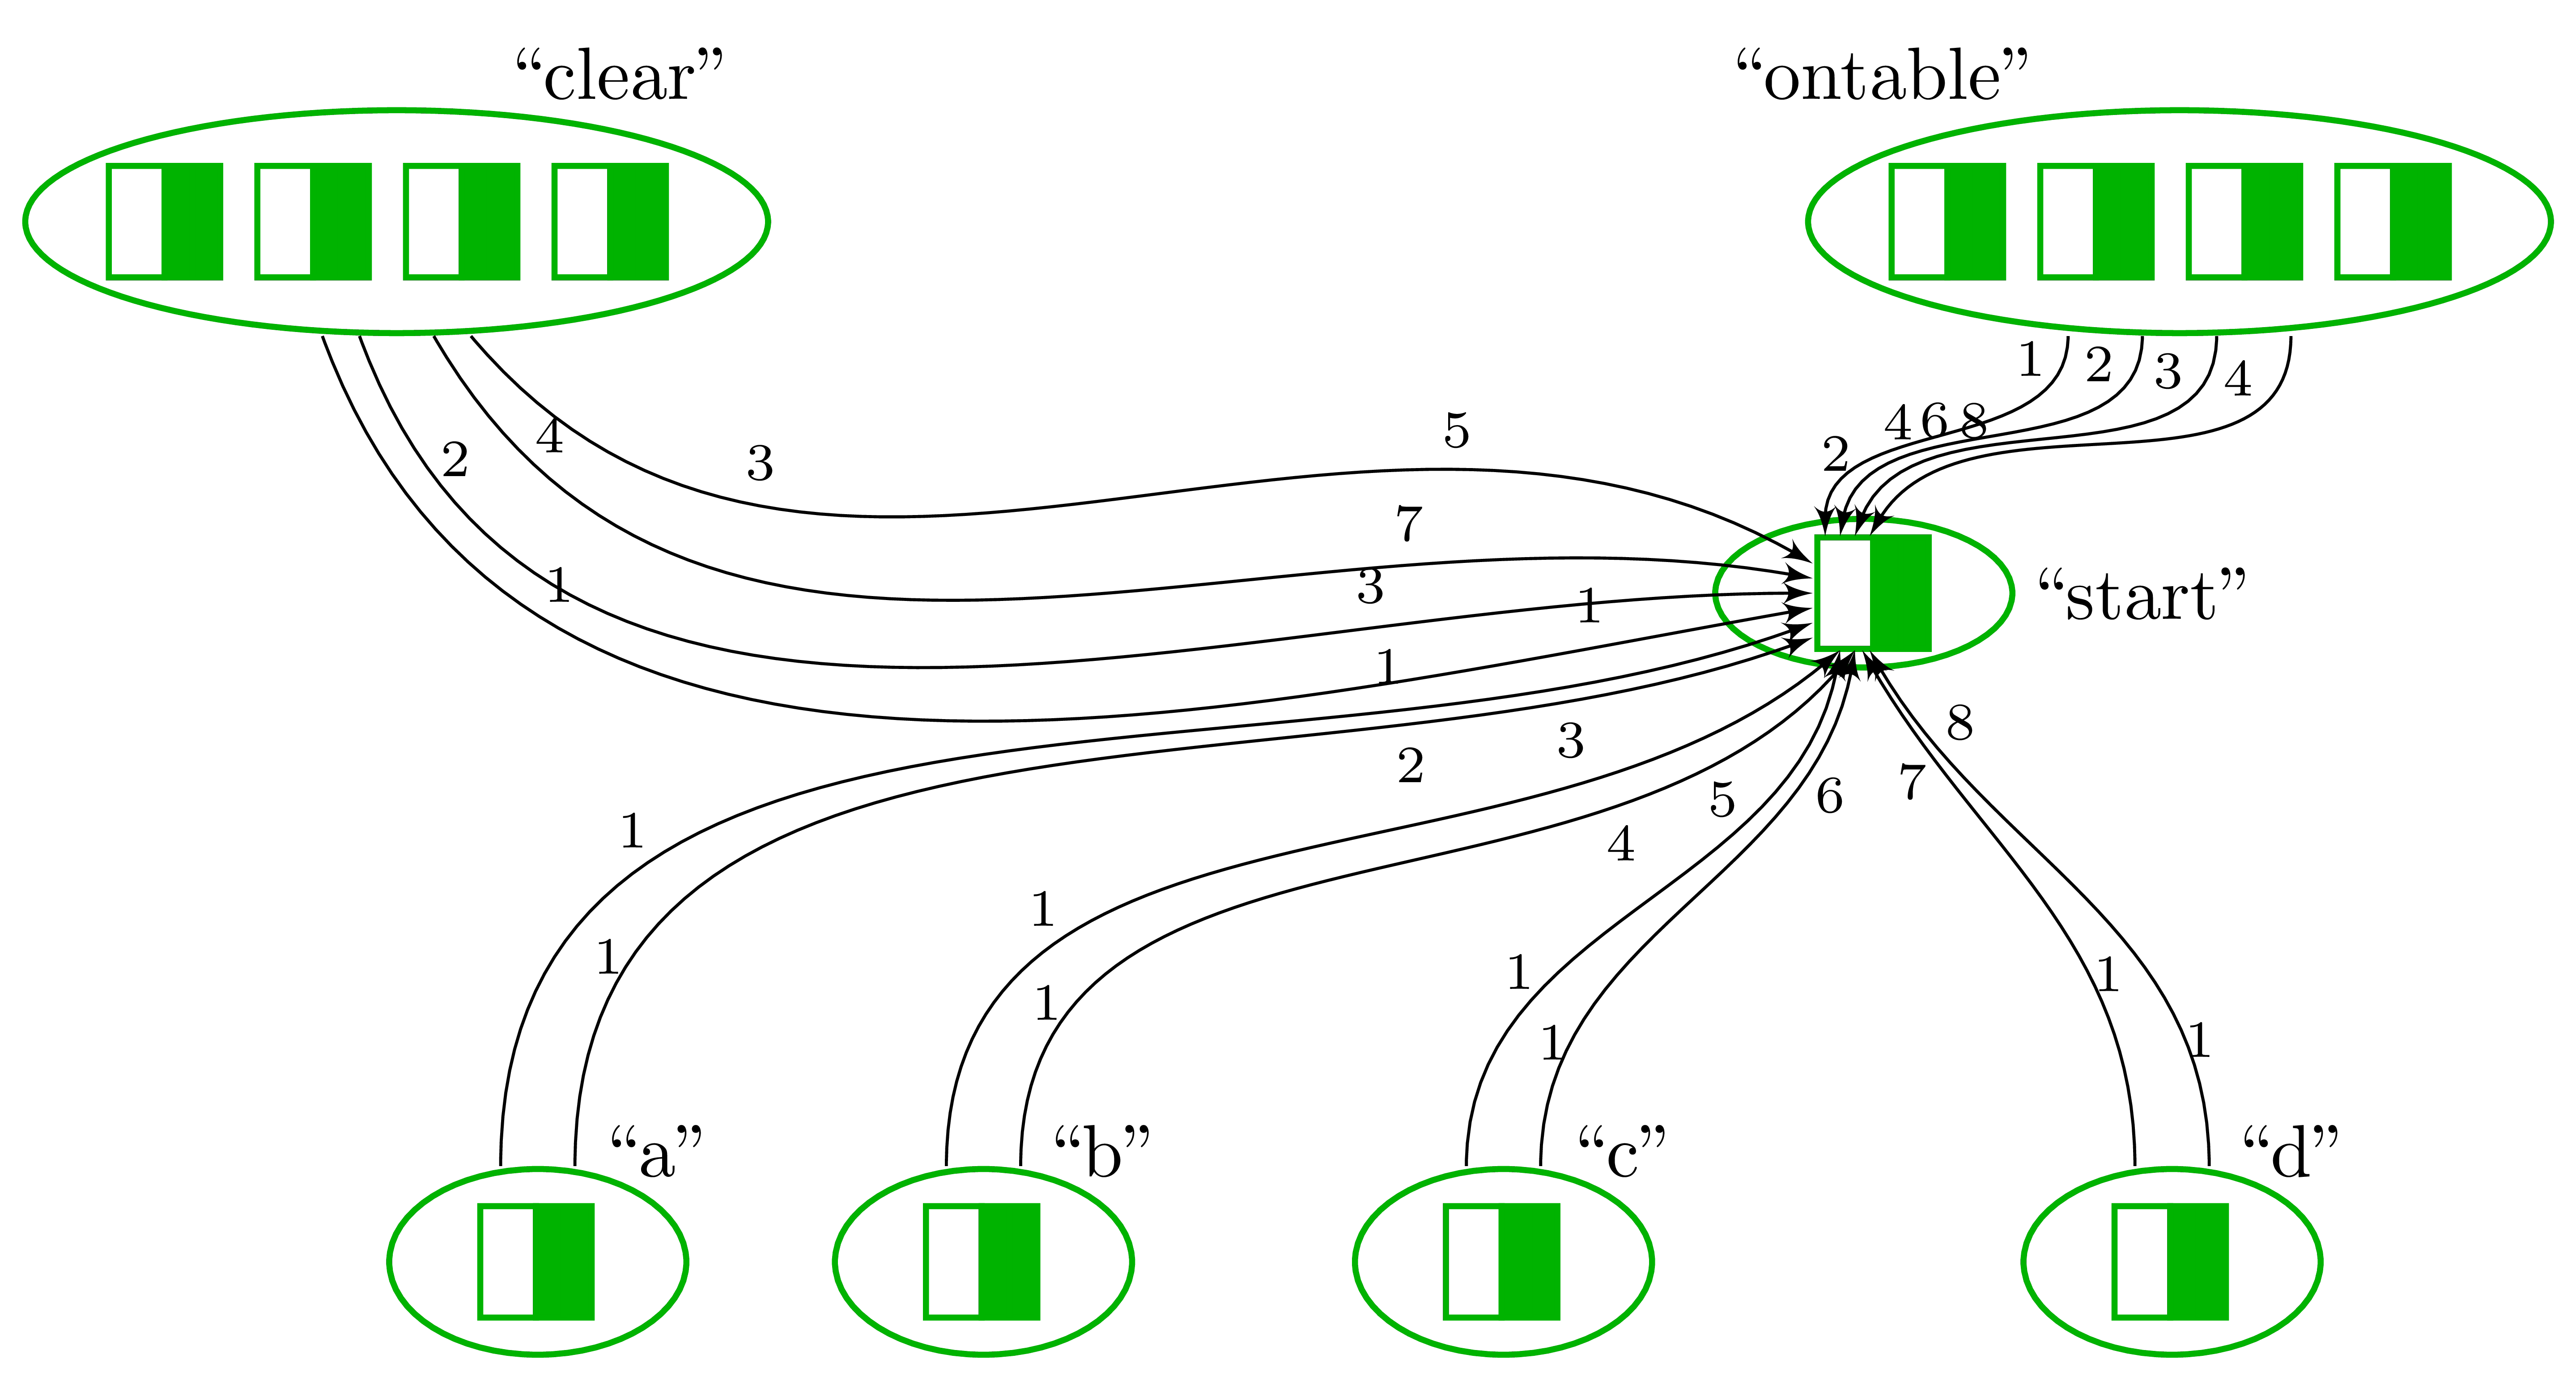
\includegraphics[width=0.75\textwidth]{plan_nets-2}
	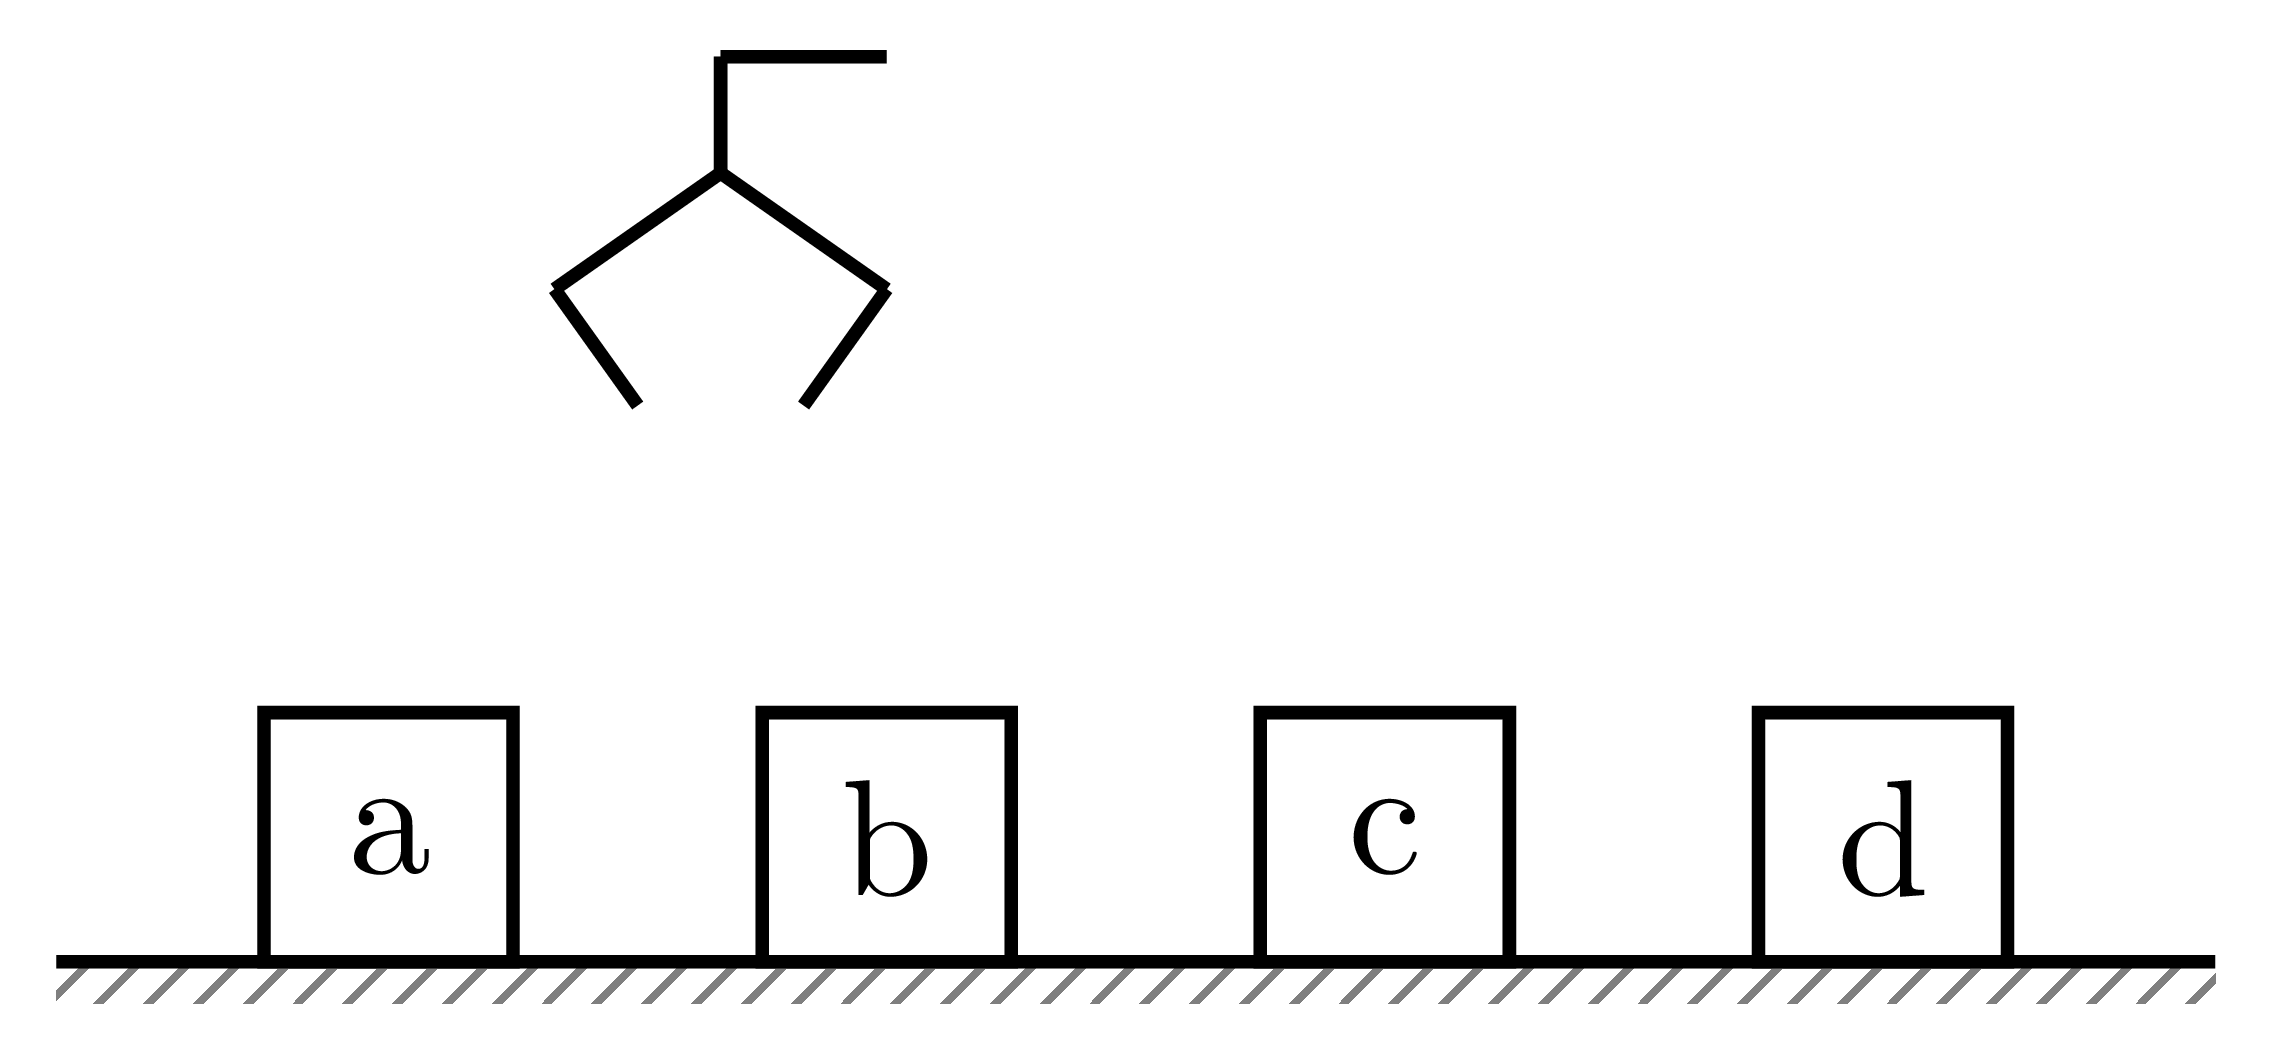
\includegraphics[width=0.6\textwidth]{block_world-1}
	\caption{Start situation: all blocks are on the table.}	
	\label{fig:start_sit}	
\end{figure}

Figure \ref{fig:goal_sit} shows the target situation in which all four blocks are stacked in a tower: block \textit{d} is located at the table, block \textit{c} --- on \textit{d}, \textit{b} --- on \textit{c}, and finally block \textit{a} is at the top. Predicate \textit{on}, which defines the relation ``located on'' may be represented in the form of a procedural causal matrix, so as to demonstrate the nonsymmetry of this relation distinctly, notwithstanding the fact that use of the object matrix has no influence on the result. Here, one causal matrix of each block also participates in the situation, and the predicate \textit{on} is represented as a node with three causal matrices, since it participates in a causal matrix of the target situation \textit{goal} in different columns with three different blocks.

\begin{figure}
	\centering
	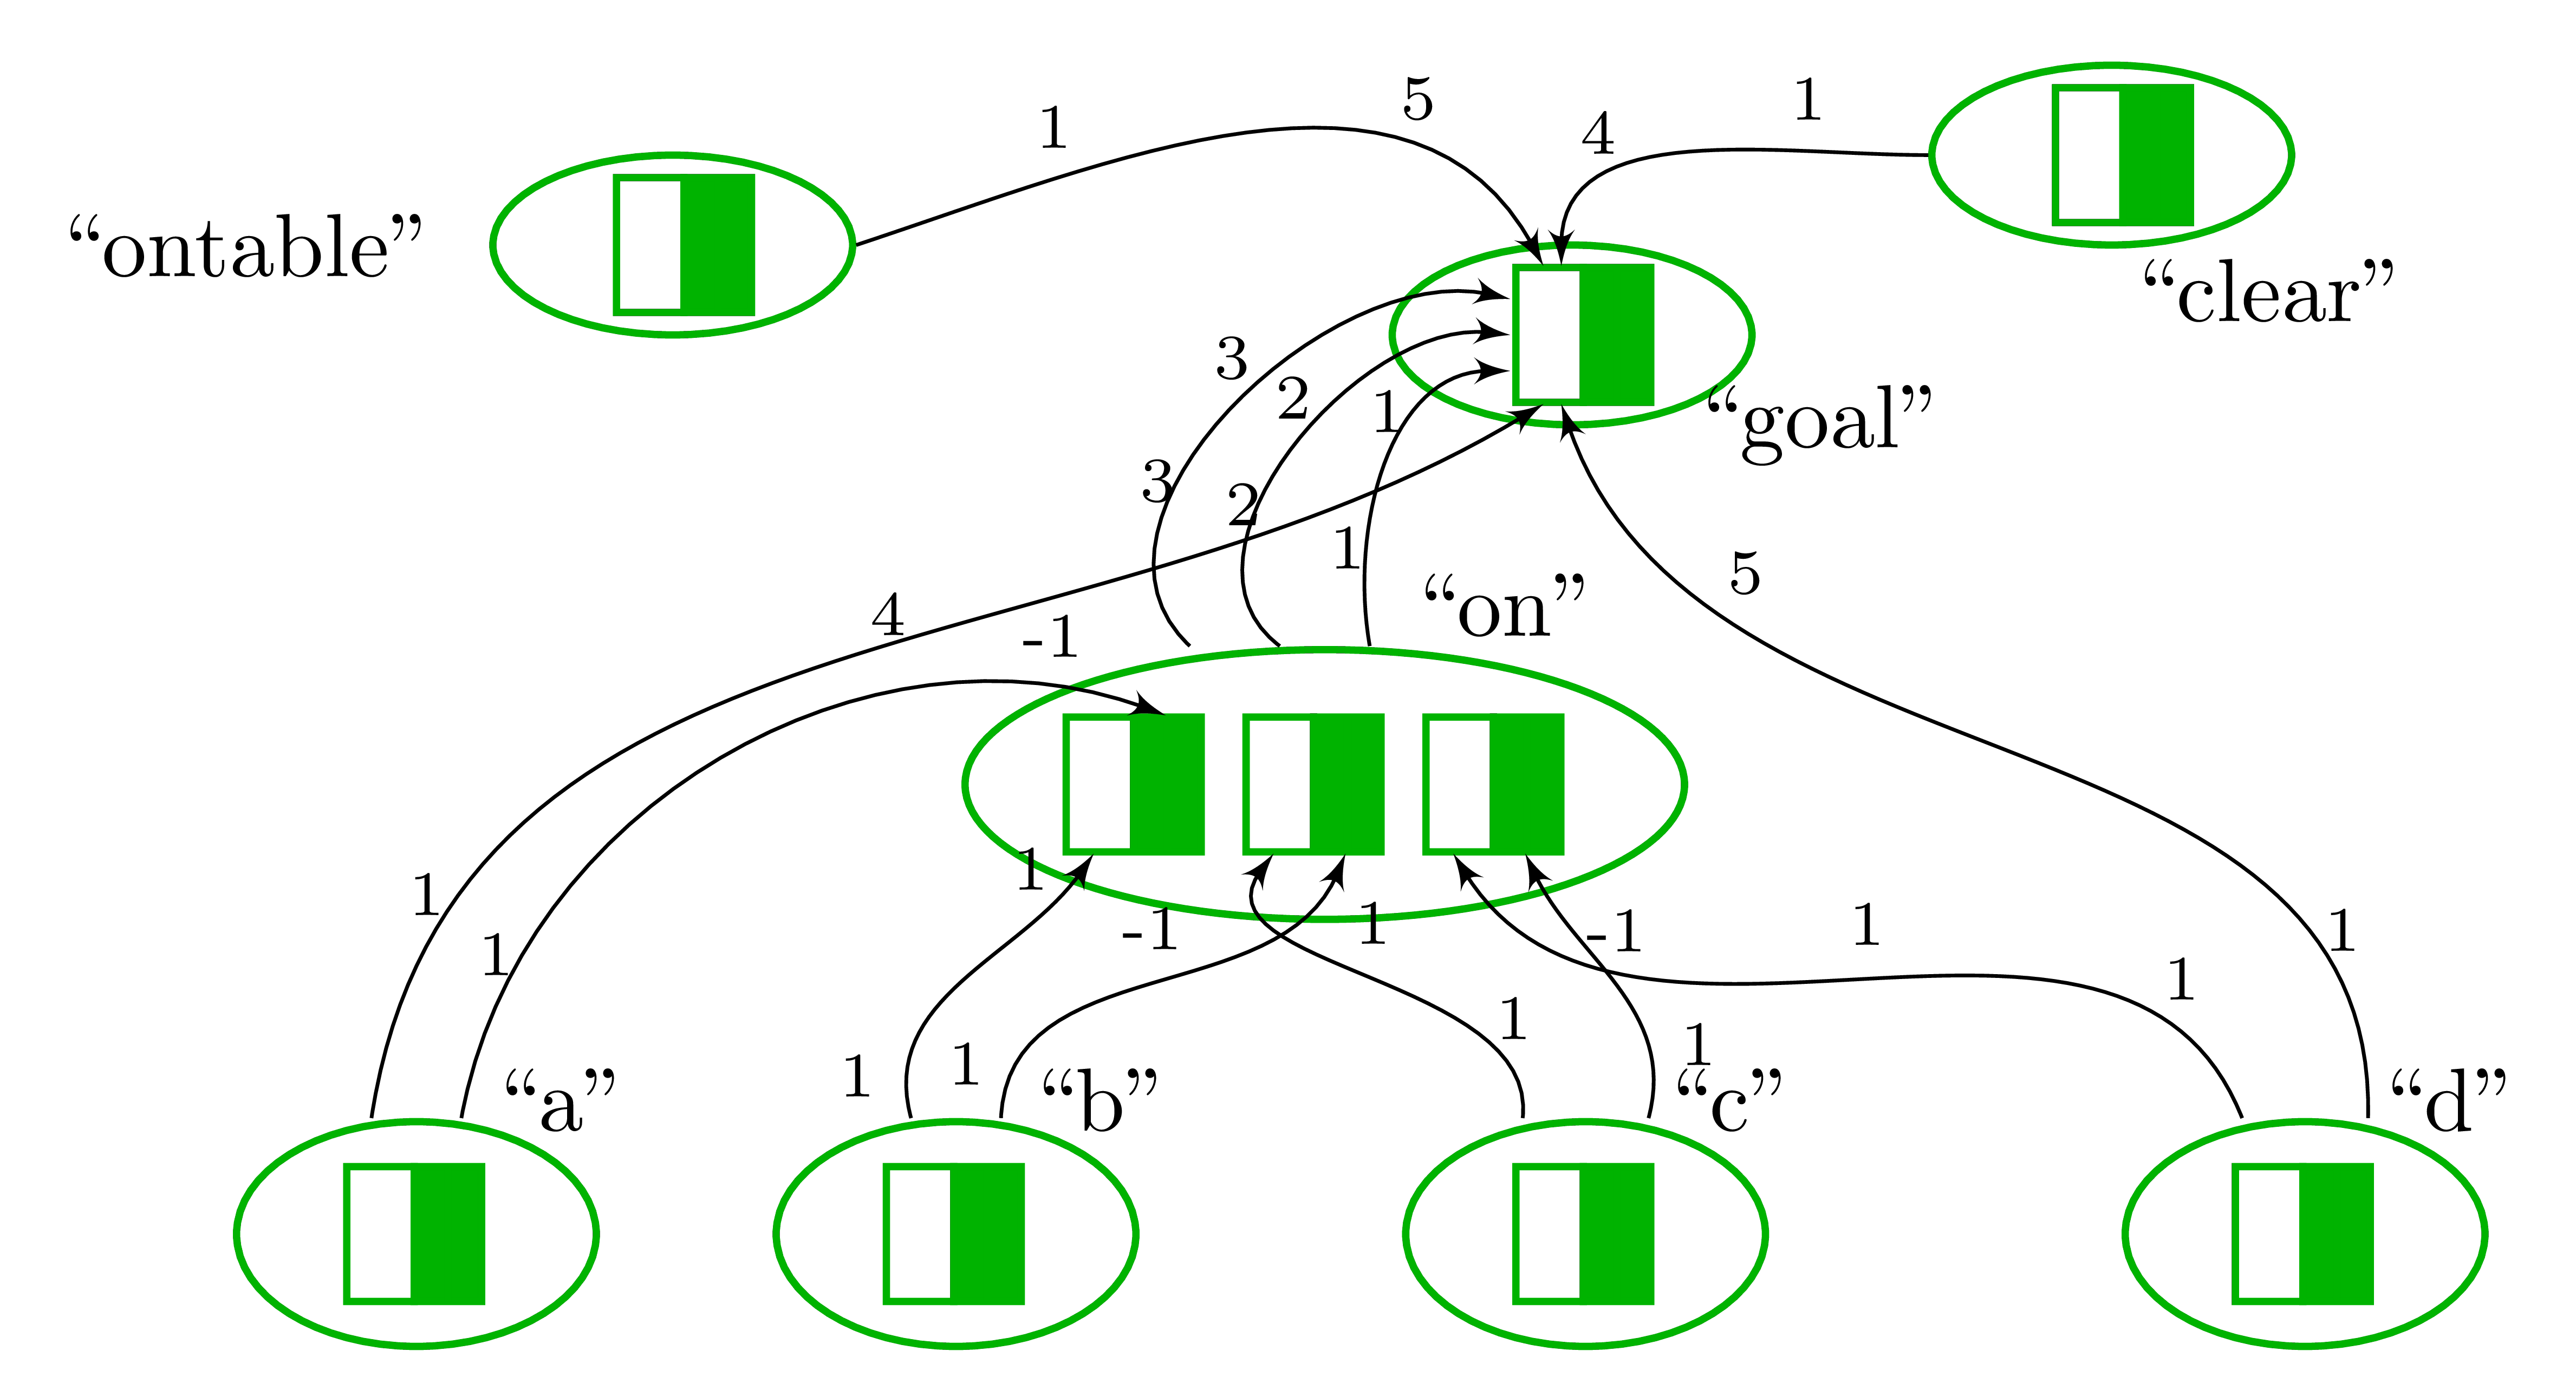
\includegraphics[width=0.73\textwidth]{plan_nets-0}
	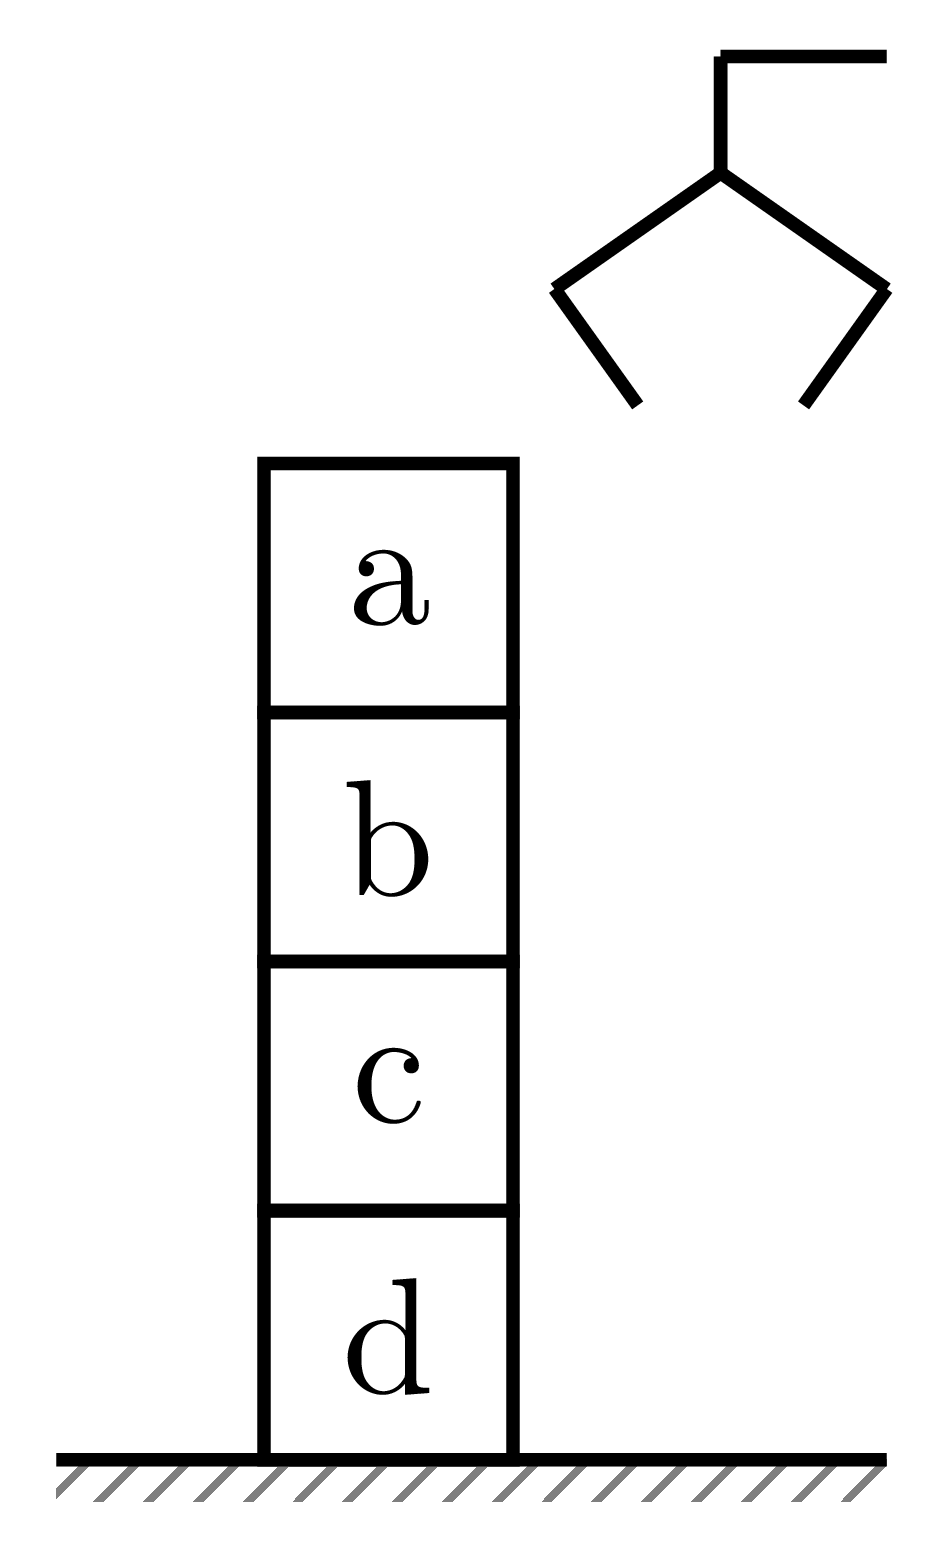
\includegraphics[width=0.23\textwidth]{block_world-0}
	\caption{Goal situation: a tower built from four blocks.}	
	\label{fig:goal_sit}	
\end{figure}

Figure \ref{fig:stack_sig} shows a fragment of a causal network for significances representing components of a procedural causal matrix of the sign \textit{stack} and relations``set-subset'' of objects (blocks), of class \textit{block} and roles in action \textit{stack}: \textit{block?x} (analog of semantic role ``object'') \textit{block?y} (analog of semantic role``directive''). It should be noted here that in the case of ``set-subset'' relation (\textit{a}$\rightarrow$\textit{block}, \textit{block}$\rightarrow$\textit{block?x}) $\epsilon_1$ edge label $v$ (index of the original matrix of the node, from which the edge is outbound $v$) possesses a special zero value indicating that any causal matrix of this node may be original. In other words, any of the blocks \textit{a}, \textit{b}, \textit{c} or \textit{d} may play the role of \textit{block?x}.

\begin{figure}
	\centering
	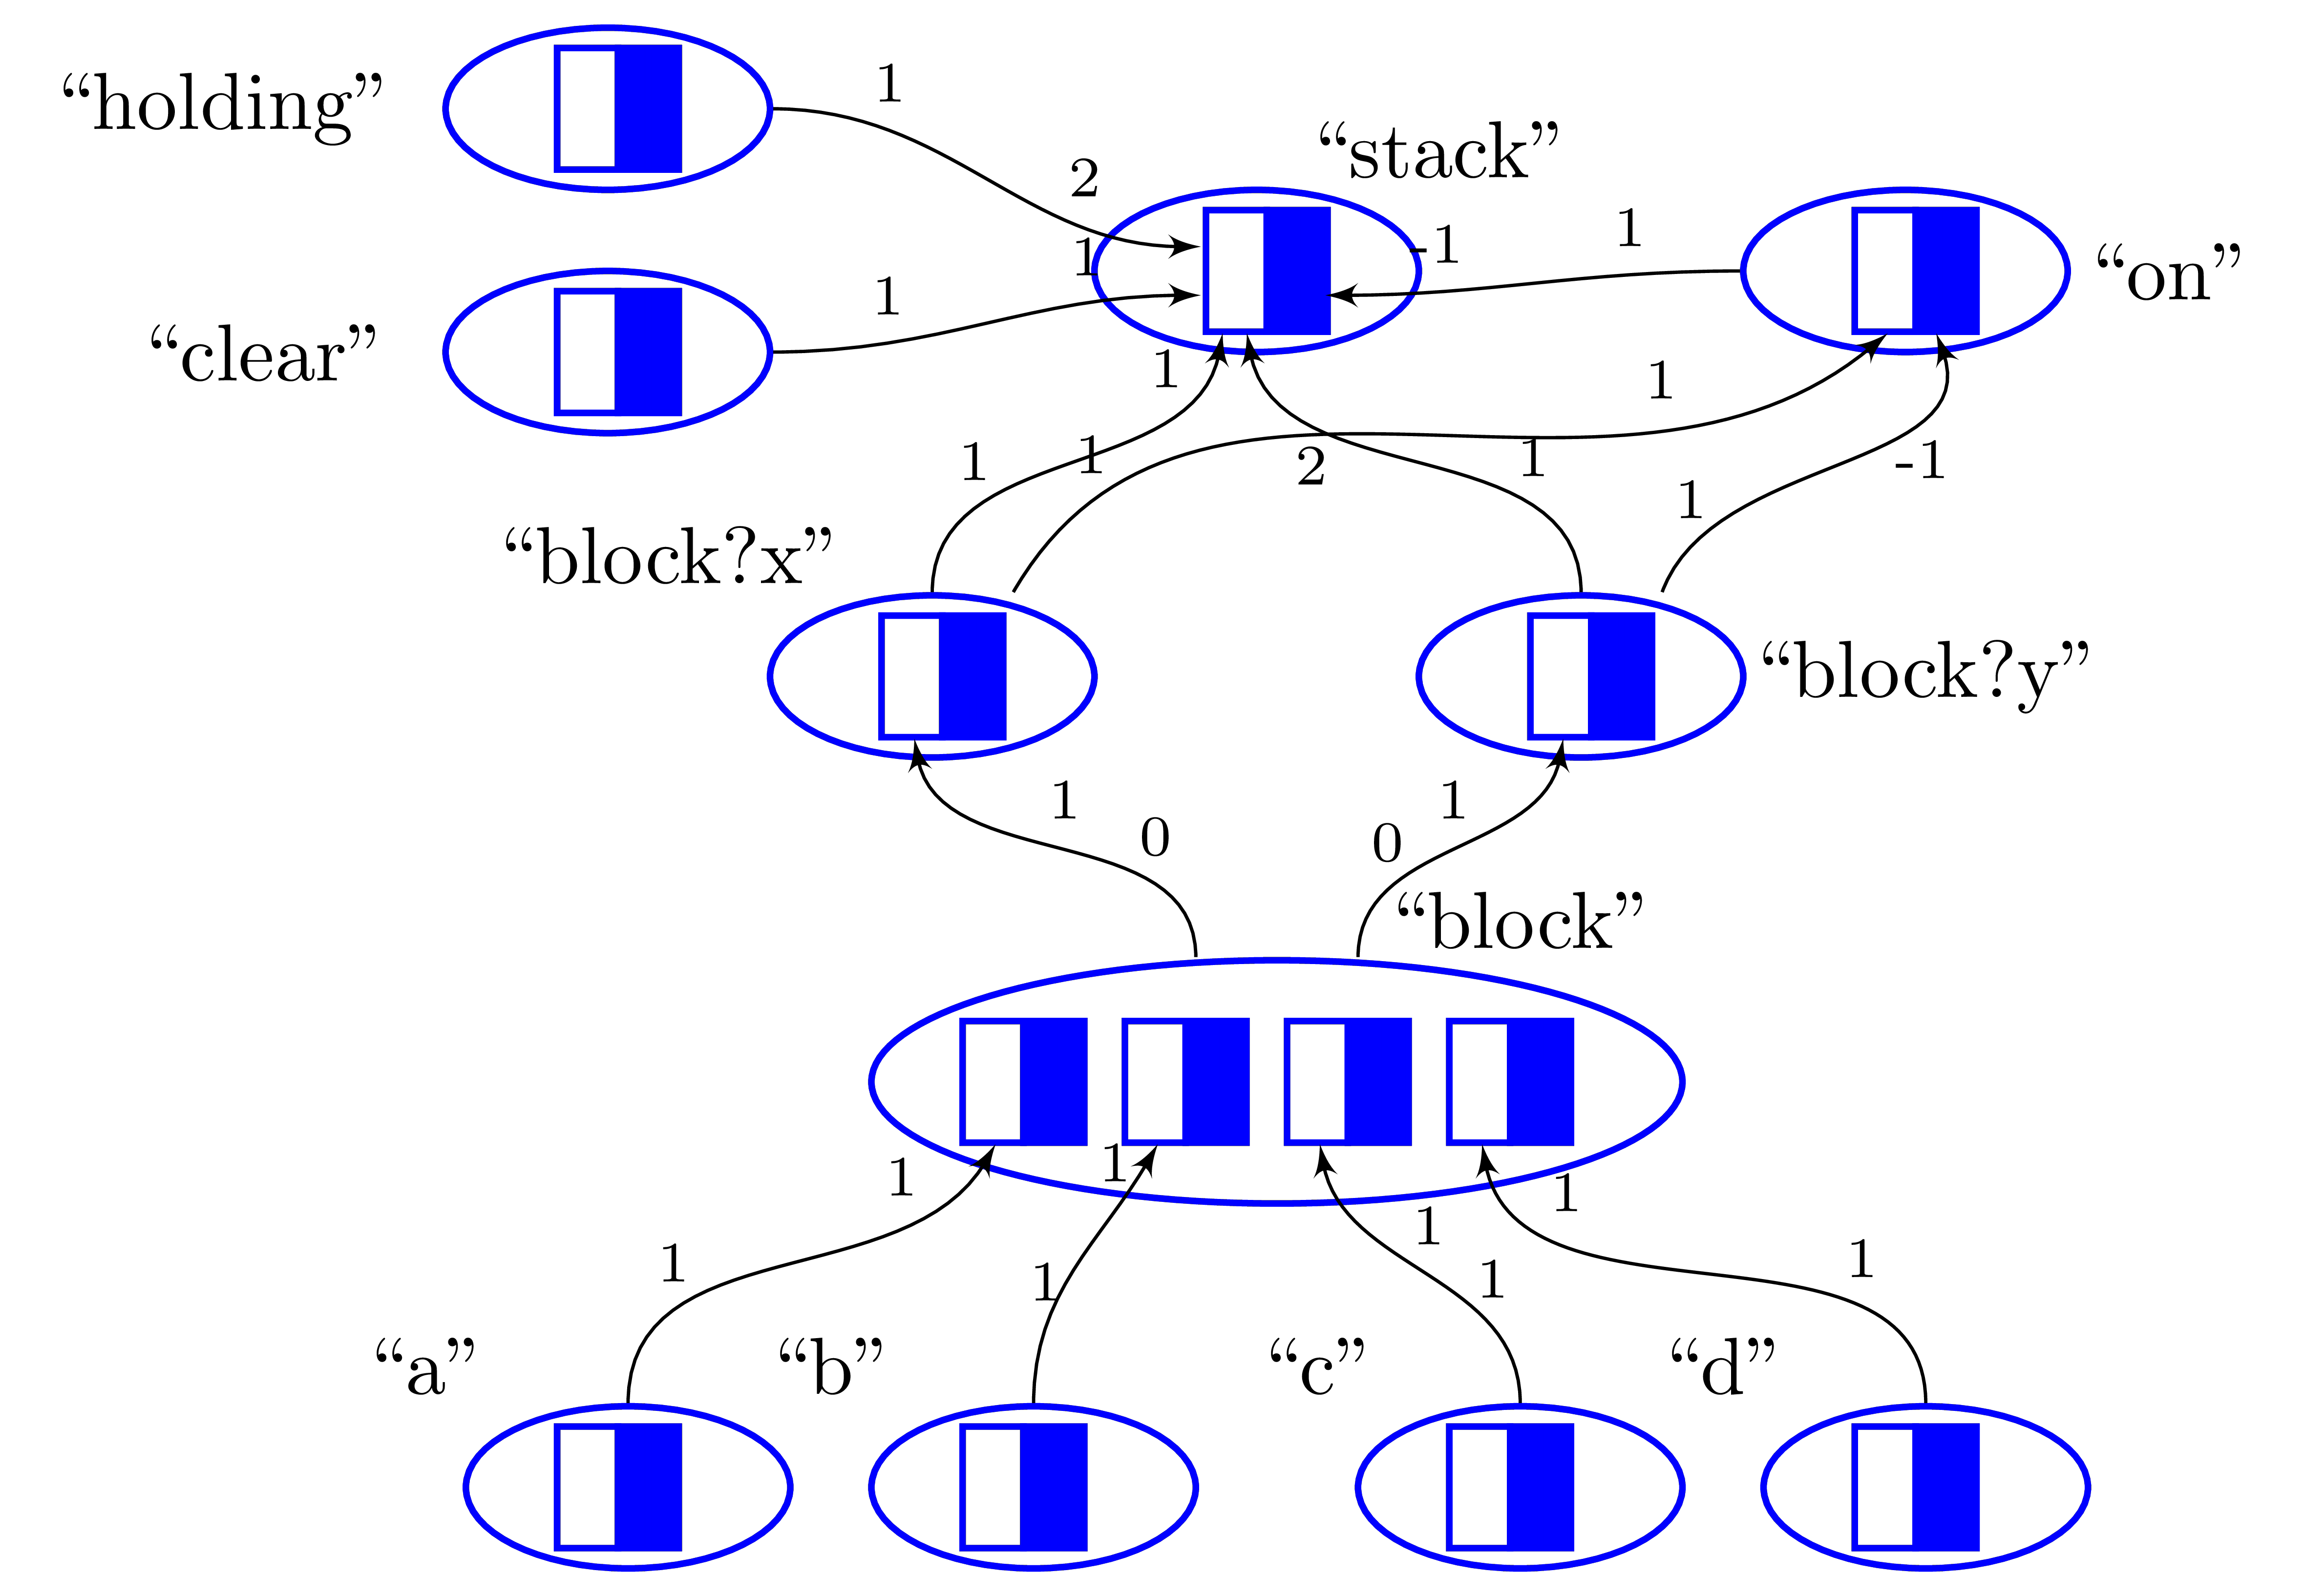
\includegraphics[width=0.7\textwidth]{plan_nets-1}
	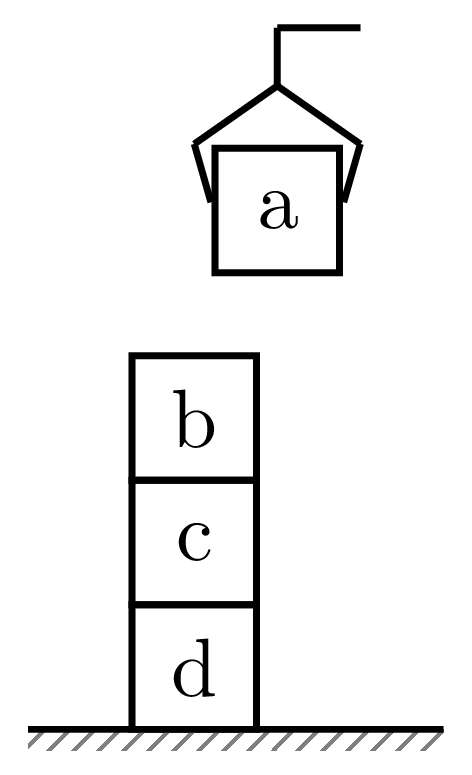
\includegraphics[width=0.27\textwidth]{block_world-2}
	\caption{Fragment of the causal network: representation of the action \textit{stack}.}	
	\label{fig:stack_sig}	
\end{figure}

Let us discuss the stages of MAP algorithm, S, M, A and P-stages, at the first iteration of the algorithm. Let us discuss the simplest case when our intelligent agent has not accumulated any experience of acting in the context of the presented problem. Due to this, at S-stage the set of precedents $\hat A_{case}$ will be empty. Taking into consideration the fact that planning is performed inversely, at the first M-stage we view the target situation as the current active prediction matrix $z_{cur}$ and propagation of activity downward from it the personal meaning network will activate set $A^*$, which coincides with the fragment shown at Figure \ref{fig:start_sit}. The set of significances $M^*$ will include the significances of the signs representing blocks \textit{a},\textit{b},\textit{c},\textit{d} --- these are all procedural signs associated with them within meaning network \textit{stack}, \textit{unstack}, \textit{pick-up}, \textit{put-down}. The left part of Figure \ref{fig:unstack_gen} shows a fragment of a causal network for significances, which includes the procedural causal matrix \textit{unstack}. To activate causal matrix \textit{unstack} by matrix \textit{a}, it is enough to use the value of three edges as constant $d_m$.

\begin{figure}
	\centering
	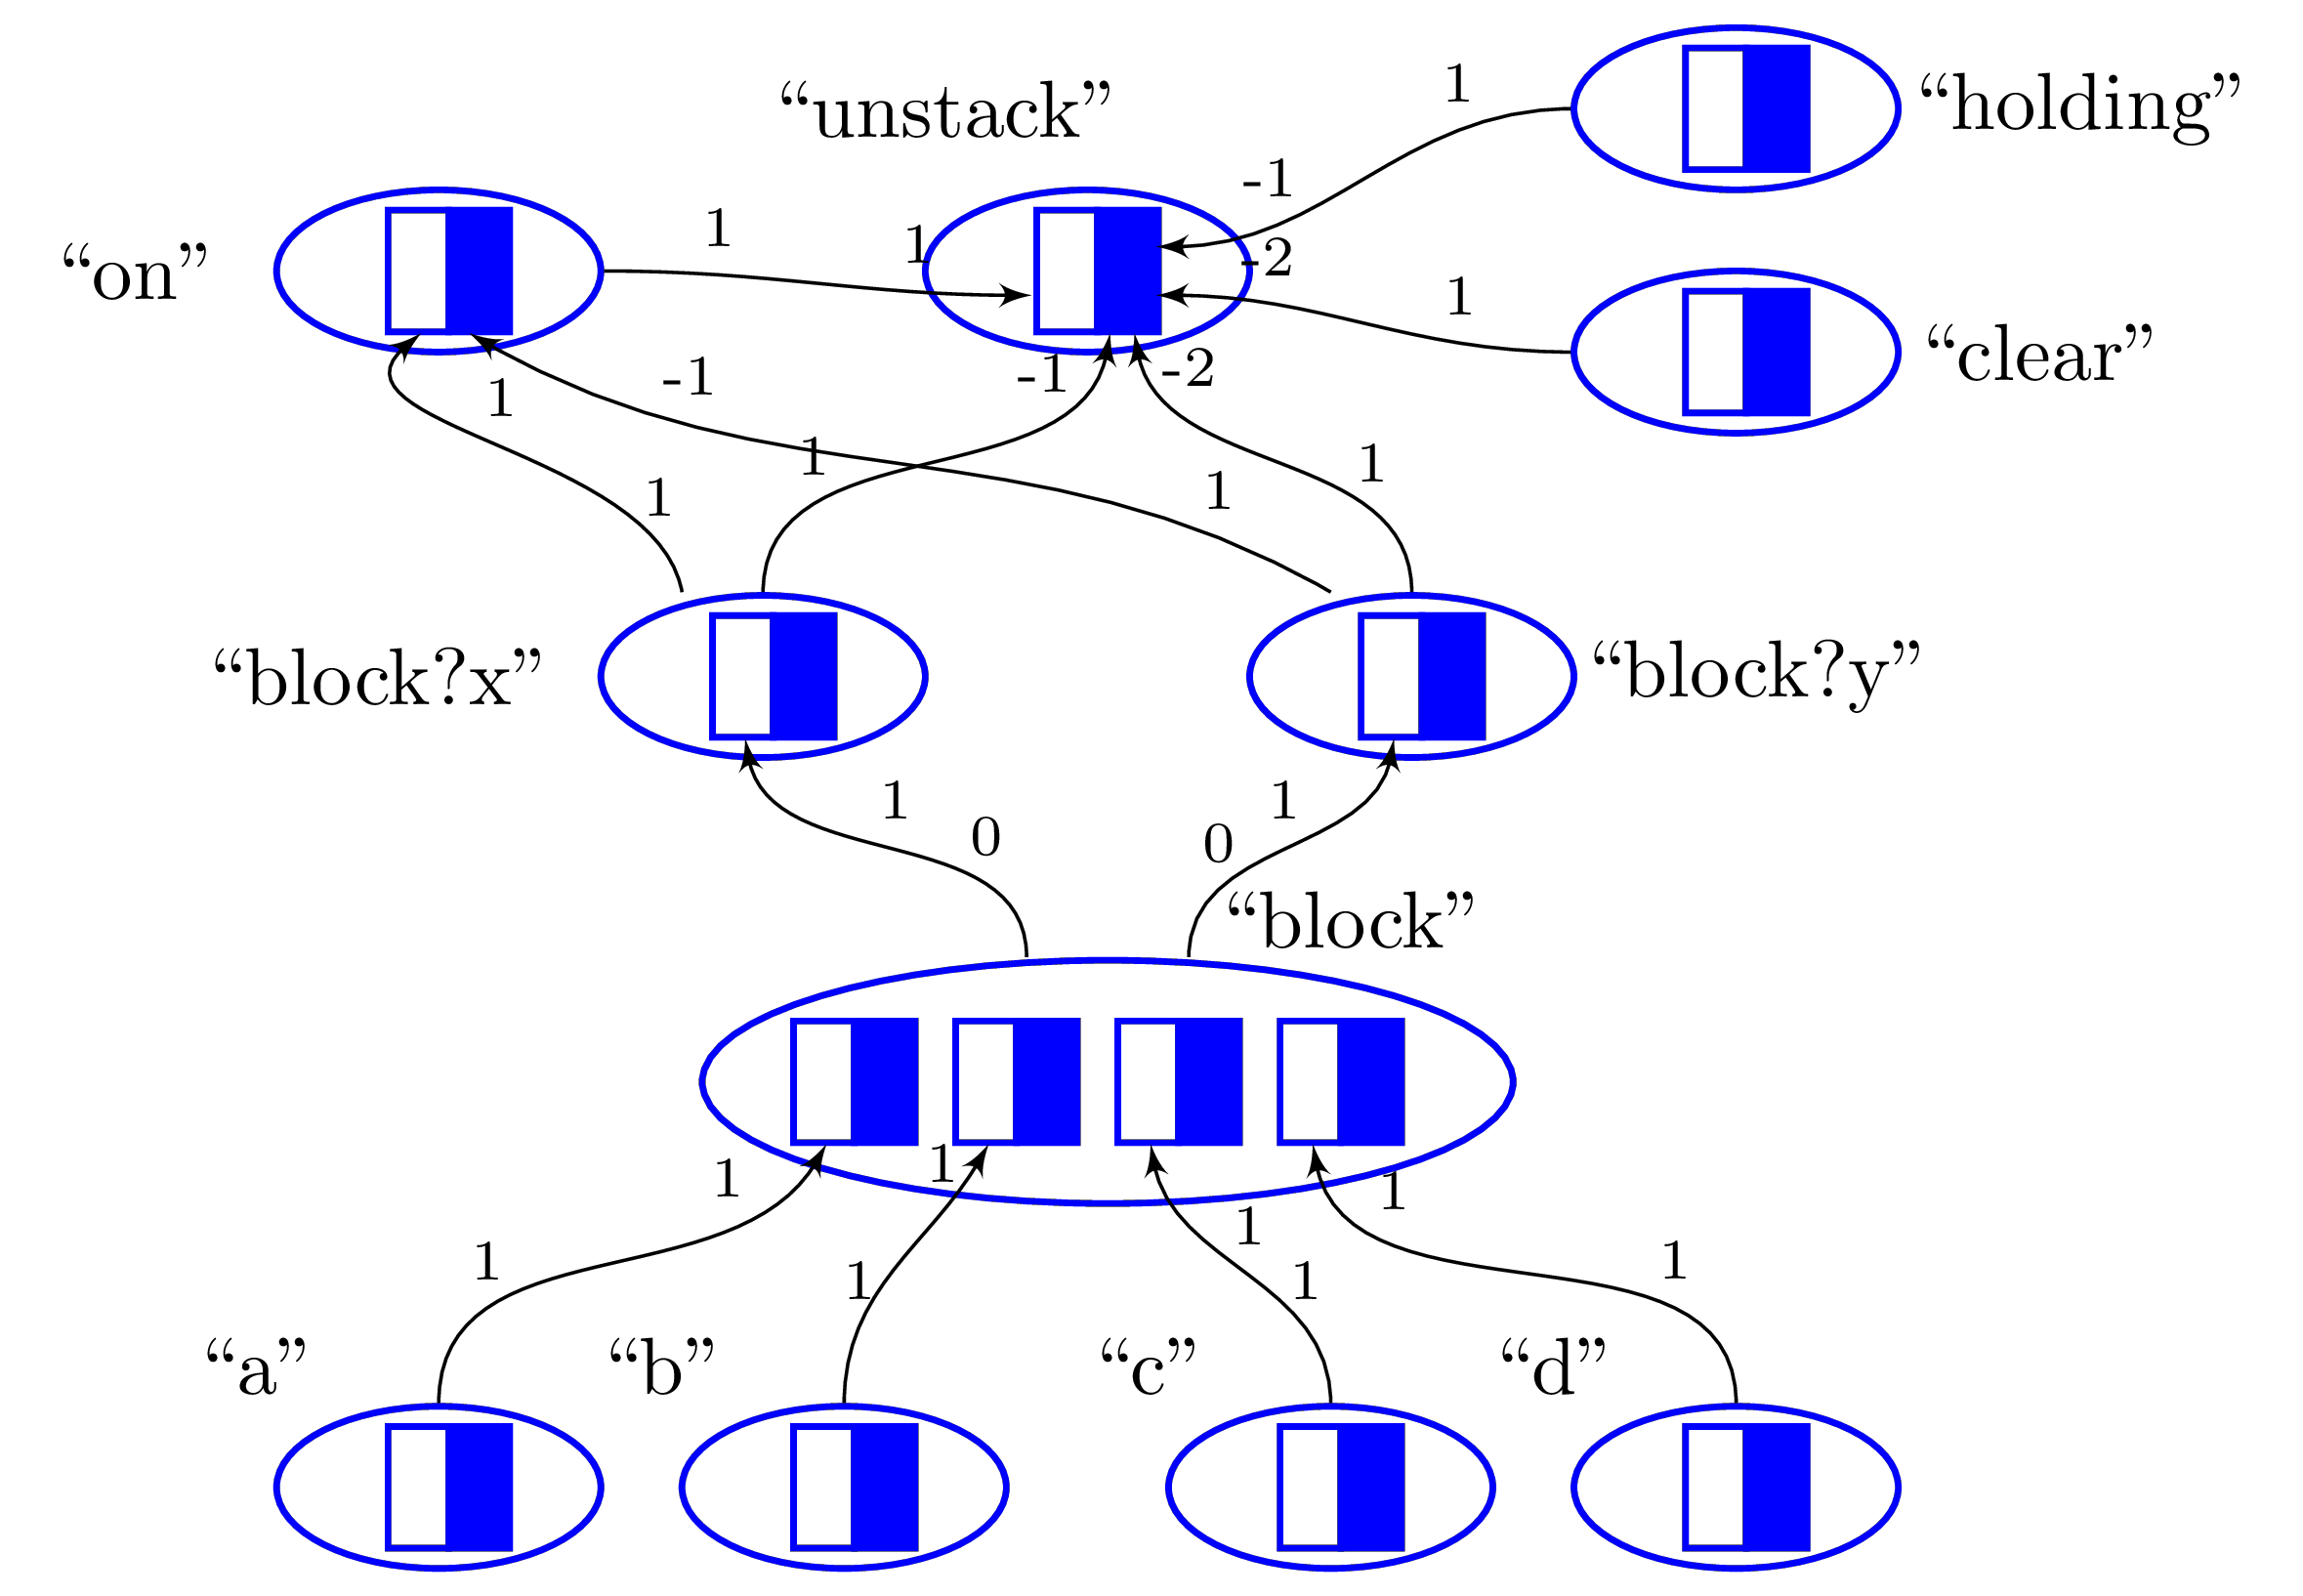
\includegraphics[width=0.48\textwidth]{plan_nets-4}
	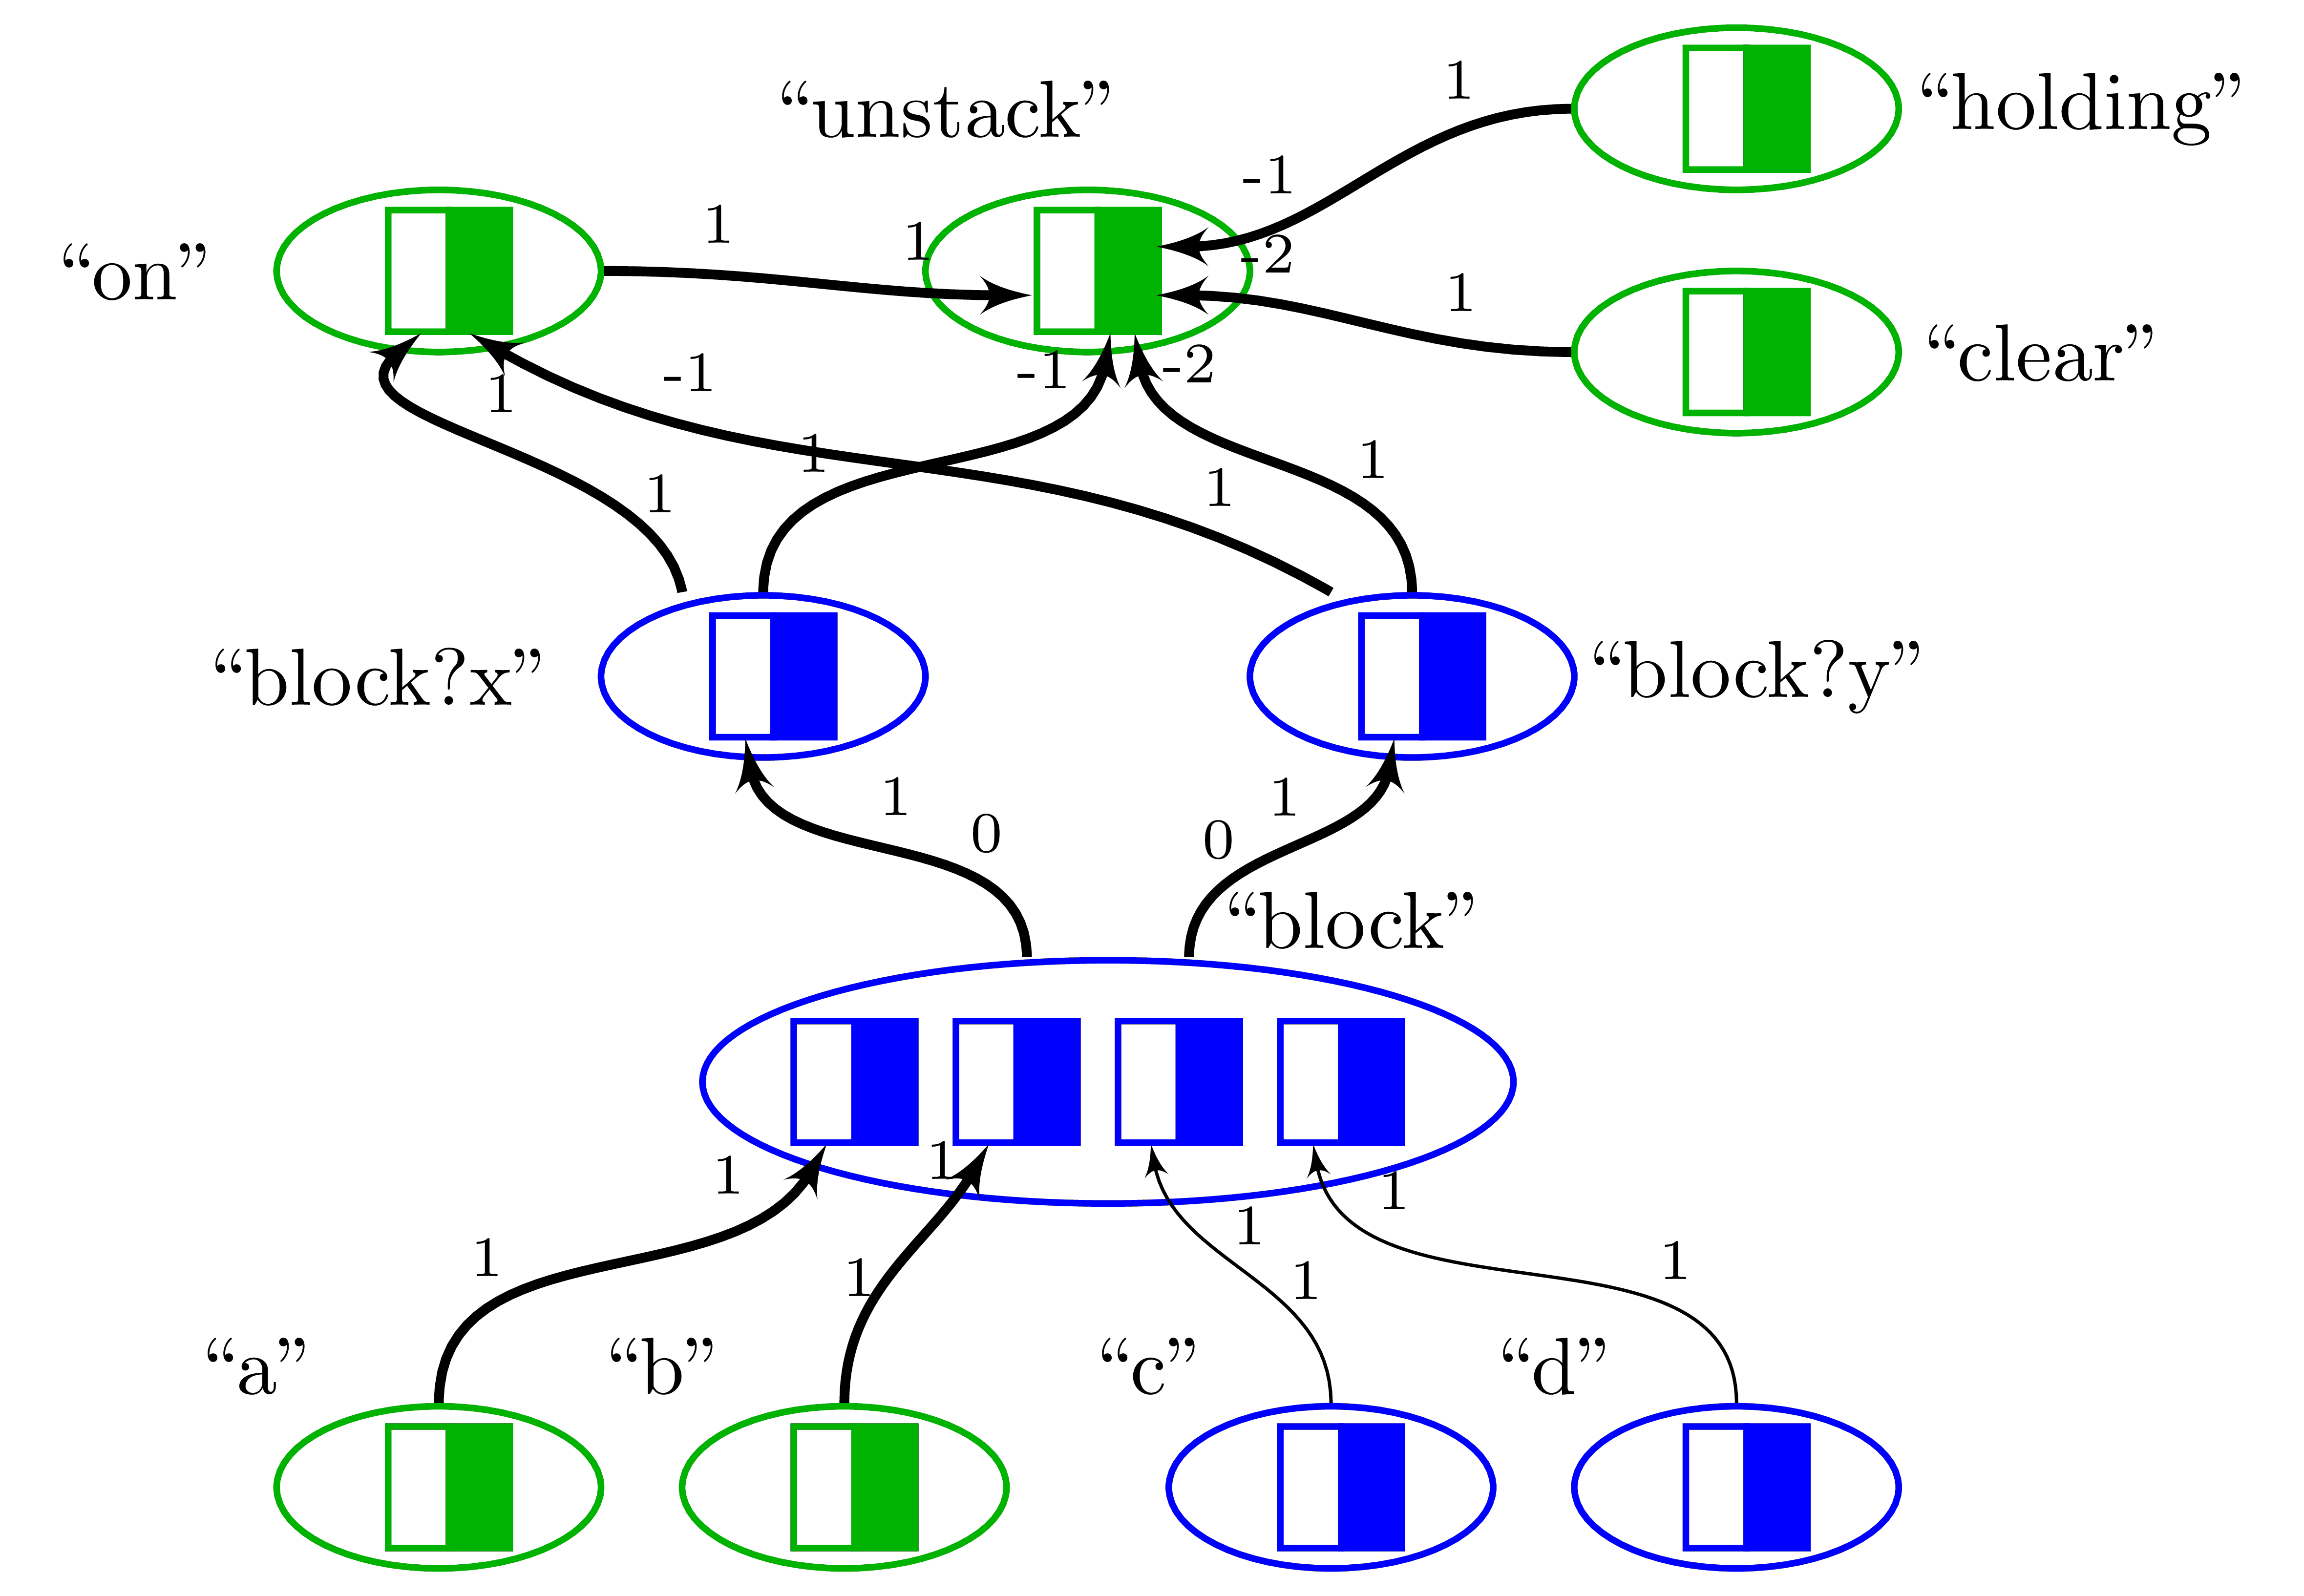
\includegraphics[width=0.48\textwidth]{plan_nets-3}
	\caption{Spreading activity in the significance network, generation of personal meaning of the sign \textit{unstack}.}	
	\label{fig:unstack_gen}	
\end{figure}

At A-stage, the generation of new causal matrices $\hat A_{gen}$ occurs in the personal meaning network by propagating activity down the network of significances. An example of this propagation, which results in a new causal matrix of sign \textit{unstack}, is shown at the right of Figure \ref{fig:unstack_gen}. The new causal matrix of the personal meaning matrix is a copy of a corresponding matrix for the network of significances, with references pointing to role signs replaced with references pointing to object non-abstract signs representing blocks. In our example, a matrix corresponding to action \textit{unstack}(\textit{a}, \textit{b}) --- remove block \textit{a} from block \textit{b} will be generated. At this stage, four matrices for each single-place actions will be generated and twelve --- for two-place actions.

A-stage is completed by testing the effects of the generated procedural matrices for applicability in the current situation, and among applicable actions those satisfying a certain meta-cognitive (heuristic) rule $\theta_a$ are selected. In our example, of all the generated variants the action \textit{unstack}(\textit{a},\textit{b}) will be the only applicable action. As a heuristic rule, the following greedy rule may be used: select actions that bring success the fastest (the new situation has more common features with the target situation).

At the end of the iteration, at P-stage, new causal matrix $z_{next}$ is generated in the personal meaning network of the sign representing the next planning situation. In our example, the new current situation will coincide with the previous with the exception that block \textit{a} is now held by a manipulator and there is nothing on block \textit{b}. A pair $\langle z_{cur}, z_a \rangle$ of the current situation's causal matrices and the selected action are added to the current $Plan_{cur}$ plan. Since the new situation does not include starting situation, we will begin a new iteration.

In our example, as the result of activity from MAP algorithm the following plan of 6 actions will be generated: \textit{pick-up}(\textit{c}), \textit{stack}(\textit{c},\textit{d}), \textit{pick-up}(\textit{b}), \textit{stack}(\textit{b},\textit{c}), \textit{pick-up}(\textit{a}), \textit{stack}(\textit{a},\textit{b}). After the agent completes working on this problem, it saves the planning precedent in its world model: it saves the initial and the final situation in the form of new signs and generates a new procedural sign, which could be called ``build a tower''. The initial situation will be the only feature in the condition column of this sign, and the target situation will be the only attribute in the effect column. After that, the intelligent agent will be able to solve the same problem by finding the required action leading to the immediate solution at S-stage. The same situation may occur while solving another problem, leading to a reduction of applicable action search space.

	
\section{Conclusion}\label{sec:concl}

In the classical symbol planning problem definition, Artificial Intelligence faces the problem of combining symbol planning algorithms with the methods of learning, which allow both to preserve planning experience and adapt to new conditions. This problem overlaps with the symbol grounding problem --- the problem of associating symbols used in the classical method of knowledge representation with real objects, processes, and properties of the external environment. These problems are very vividly manifested in the area of implementing learning robotics systems, for which it is important to associate the symbols used in conceptual planning and the data obtained by sensors. It should be noted that when a complex technical system is presented with a planning problem in a broad spectrum of conditions, including cooperative ones, approaches using a preset, albeit replenished knowledge base prove to be inefficient. A method of representing knowledge serving as the basis for the control functions of an intelligent agent, should inherently support the possibility to associate symbols with sensor data, as well as support the representation of both internal information and generalized information coordinated between other participants of the group. This article solves the said problems by using a sign world model. We present an original planning method (MAP algorithm), which uses and maintains the precedent information in the process of plan generation. The four-component world model component (sign) used allows coding both the information of the external environment and internal attributes, motivation and need properties, as well as general collective knowledge. The algorithm presented may also be used for the generation of cooperative plans. To demonstrate MAP Planner, a model example of the generation of the plan for one of the ``block world'' problems is presented. Software support and model experiments may as well be found at \href{https://github.com/cog-isa/map-planner}{https://github.com/cog-isa/map-planner}.

\section*{Acknowledgment}
This work was supported by the Russian Foundation for Basic Research (Project No. 16-37-60055).

\section*{References}

\bibliography{sign_planning}

\end{document}